\batchmode


\documentclass[11pt,a4paper,oneside,onecolumn]{book}
\RequirePackage{ifthen}


\usepackage{epsfig} 
\usepackage{latexsym,amsfonts,amssymb,amstext,amsthm,float,amsmath,dsfont}
\usepackage[spanish]{babel}    
\usepackage{ucs}
\usepackage[utf8x]{inputenc}
\usepackage{alltt}
\usepackage{html}
\usepackage{makeidx}
\usepackage{hyperref}


\usepackage[usenames,dvipsnames]{xcolor}
\usepackage{listings}
\lstloadlanguages{Ruby}
\lstset{%
backgroundcolor=\color{GreenYellow},
basicstyle=\ttfamily\color{black},
commentstyle = \ttfamily\color{red},
keywordstyle=\ttfamily\color{blue},
stringstyle=\color{orange}}


\voffset -10 mm
\topmargin 0 mm
\headheight 0 mm
\headsep 0 mm


\textheight 256 mm


\oddsidemargin -5.4 mm
\evensidemargin -5.4 mm


\textwidth 17 cm
\columnsep 10 mm

%
\providecommand{\datetofill}{\rule{5mm}{.1pt}/\rule{5mm}{.1pt}/\rule{10mm}{.1pt}} 

%
\providecommand{\infinity}{\infty} 

%
\providecommand{\ici}[1]{\index{#1}} 

%
\providecommand{\perlcookbook}[2]{\htmladdnormallink{#1}{http://docstore.mik.ua/orelly/perl/cookbook/#2}} 

%
\providecommand{\pci}[1]{\index{Práctica!#1}} 

%
\providecommand{\ci}[1]{\index{#1}#1} 

%
\providecommand{\cei}[1]{\index{#1}\emph{#1}} 

%
\providecommand{\ceis}[2]{\index{#2}\emph{#1}} 

%
\providecommand{\tei}[1]{ {\tt #1} }  %{\index{#1}{{\tt #1}}}

%
\providecommand{\htei}[1]{ #1 }  %{\index{#1}}

%
\providecommand{\teis}[2]{\index{#2}{{\tt #1}}} 

%
\providecommand{\xsub}[1]{\index{XSUB!{\tt #1}}
   {\tt #1}
  } 

%
\providecommand{\typemap}[1]{\index{typemap!{\tt #1}}
   {\tt #1}
  } 

%
\providecommand{\api}[1]{\index{Perl API!{\tt #1}}
   {\tt #1}
  } 

%
\providecommand{\hueco}[1]{\underline{\hspace{#1cm}}} 

%
\providecommand{\parrafo}[1]{ 
  \paragraph{#1}
  \begin{tabular}{c}
  \end{tabular}
} 

%
\providecommand{\sectionpractica}[1]{\section{Práctica: #1}
   \index{Práctica!#1}
  } 

%
\providecommand{\subsectionpractica}[1]{\subsection{Práctica: #1}
   \index{Práctica!#1}
  } 

%
\providecommand{\subsubsectionpractica}[1]{\subsubsection{Práctica: #1}
   \index{Práctica!#1}
  } 

%
\providecommand{\sectionejercicio}[1]{\section{Ejercicio: #1}
   \index{Ejercicio!#1}
  } 

%
\providecommand{\parrafopractica}[1]{ 
  \paragraph{Práctica: #1}
  \begin{tabular}{c}
  \end{tabular}

   \index{Práctica!#1}
  } 

%
\providecommand{\subsectionejercicio}[1]{\subsection{Ejercicio: #1}
   \index{Ejercicio!#1}
  } 

%
\providecommand{\subsubsectionejercicio}[1]{\subsubsection{Ejercicio: #1}
   \index{Ejercicio!#1}
  } 

%
\providecommand{\subsectionrepaso}[1]{\subsection{Repaso: #1}
   \index{Repaso!#1}
  } 

%
\providecommand{\eref}[1]{\externalref{#1} \cite{CasianoIntroAPerl}} 

%
\providecommand{\regexpg}{\htmladdnormallink{{\tt Regexp::Grammars}}
 {http://search.cpan.org/perldoc?Regexp::Grammars}} 

%
\providecommand{\rgsec}[2]{\htmladdnormallink{#1}
 {http://search.cpan.org/~dconway/Regexp-Grammars/lib/Regexp/Grammars.pm\##2}} 



\newtheorem{definition}{Definición}[section] 
\newtheorem{theorem}{Teorema}[section] 
\newtheorem{algorithm}{Algoritmo}[section] 
\newtheorem{program}{Programa}[section] 
\newtheorem{exercise}{Ejercicio}[section] 


\newtheorem{example}{Ejemplo}[section] 
\newtheorem{execution}{Ejecución}[section] 
\newtheorem{listing}{Listado}[section] 
\newtheorem{advice}{Consejo}[section] 
\newtheorem{scheme}{Esquema}[section] 


%
\newenvironment{unicodeverb}{\begin{verbatim}
}
{\end{verbatim}
} 

%
\providecommand{\modern}{{\it Modern Perl}} 

%
\providecommand{\lhp}[2]{\htmladdnormallink{#1}
{http://nereida.deioc.ull.es/~lhp/perlexamples/node#2.html}} 

%
\providecommand{\man}[1]{\htmladdnormallink{{\tt #1}}
{http://manpages.debian.net/cgi-bin/man.cgi?query=#1}} 

%
\providecommand{\manuk}[1]{\htmladdnormallink{{\tt #1}}
{http://unixhelp.ed.ac.uk/CGI/man-cgi?#1}} 

%
\providecommand{\mandragonfly}[1]{\htmladdnormallink{{\tt #1}}
{http://leaf.dragonflybsd.org/cgi/web-man?command=#1&section=ANY}} 

%
\providecommand{\manopenbsd}[1]{\htmladdnormallink{{\tt #1}}
{http://www.openbsd.org/cgi-bin/man.cgi?query=#1}} 

%
\providecommand{\link}[2]{\htmladdnormallink{#1}
{#2}} 

%
\providecommand{\cpan}[1]{\htmladdnormallink{{\tt #1}}
 {http://search.cpan.org/perldoc?#1}} 

%
\providecommand{\githelp}[2]{\htmladdnormallink{#1}
 {http://help.github.com/#2/}} 

%
\providecommand{\github}{\htmladdnormallink{GitHub}
 {http://help.github.com}}%
\providecommand{\npm}{\htmladdnormallink{{\tt npm}}
 {https://npmjs.org/}} 

%
\providecommand{\npmdoc}[1]{\htmladdnormallink{{\tt #1}}
 {https://npmjs.org/doc/#1.html}} 

%
\providecommand{\ebnfparser}{\htmladdnormallink{{\tt ebnf-parser}}
 {https://github.com/zaach/ebnf-parser}} 

%
\providecommand{\markdown}{\htmladdnormallink{{\tt markdown}}
 {http://daringfireball.net/projects/markdown/syntax}} 

%
\providecommand{\rake}{\htmladdnormallink{{\tt Rake}}
 {http://rake.rubyforge.org/}} 

%
\providecommand{\rbp}{\htmladdnormallink{{\tt Ruby Best Practices}}
 {http://www.humbug.in/docs/ruby-best-practices/index.html} \cite{RBP}} 

%
\providecommand{\rspec}{\htmladdnormallink{{\tt RSpec}}
 {http://rspec.info/}} 

%
\providecommand{\rubyforge}[2]{\htmladdnormallink{#1}
 {http://rake.rubyforge.org/classes/#2}} 

%
\providecommand{\rubygems}{\htmladdnormallink{{\tt RubyGems.org}}
 {https://rubygems.org/}} 

%
\providecommand{\gem}{\htmladdnormallink{{\tt gems}}
 {http://docs.rubygems.org/read/book/2}} 

%
\providecommand{\webrick}{\htmladdnormallink{{\tt Webrick}}{http://naupacto.com/rubydoc/guiaWEBrick/index.html}}%
\providecommand{\shotgun}{\htmladdnormallink{{\tt Shotgun}}{http://ruby.about.com/od/sinatra/a/sinatra5.htm}} 

%
\providecommand{\rubymod}[1]{\index{#1}\htmladdnormallink{{\tt #1}}
 {http://www.ruby-doc.org/core-1.9.3/#1.html}} 

%
\providecommand{\String}{\htmladdnormallink{{\tt String}}
 {http://www.ruby-doc.org/core-1.9.3/String.html}} 

%
\providecommand{\Symbol}{\htmladdnormallink{{\tt Symbol}}
 {http://www.ruby-doc.org/core-1.9.3/Symbol.html}} 

%
\providecommand{\Proc}{\htmladdnormallink{{\tt Proc}}
 {http://www.ruby-doc.org/core-1.9.3/Proc.html}} 

%
\providecommand{\Method}{\htmladdnormallink{{\tt Method}}
 {http://www.ruby-doc.org/core-1.9.3/Method.html}} 

%
\providecommand{\UnboundMethod}{\htmladdnormallink{{\tt UnboundMethod}}
 {http://www.ruby-doc.org/core-1.9.3/UnboundMethod.html}} 

%
\providecommand{\Binding}{\htmladdnormallink{{\tt Binding}}
 {http://www.ruby-doc.org/core-1.9.3/Binding.html}} 

%
\providecommand{\Kernel}{\htmladdnormallink{{\tt Kernel}}
 {http://www.ruby-doc.org/core-1.9.3/Kernel.html}} 

%
\providecommand{\BasicObject}{\htmladdnormallink{{\tt BasicObject}}
 {http://www.ruby-doc.org/core-1.9.3/BasicObject.html}} 

%
\providecommand{\Object}{\htmladdnormallink{{\tt Object}}
 {http://www.ruby-doc.org/core-1.9.3/Object.html}} 

%
\providecommand{\Enumerable}{\htmladdnormallink{{\tt Enumerable}}
 {http://www.ruby-doc.org/core-1.9.3/Enumerable.html}} 

%
\providecommand{\Class}{\htmladdnormallink{{\tt Class}}
 {http://www.ruby-doc.org/core-1.9.3/Class.html}} 

%
\providecommand{\Module}{\htmladdnormallink{{\tt Module}}
 {http://www.ruby-doc.org/core-1.9.3/Module.html}} 

%
\providecommand{\rubycoreclassmethod}[2]{\index{#1}\htmladdnormallink{{\tt #1}}
 {http://www.ruby-doc.org/core-1.9.3/#2.html\#method-c-#1}} 

%
\providecommand{\rubycoreinstancemethod}[2]{\index{#1}\htmladdnormallink{{\tt #1}}
 {http://www.ruby-doc.org/core-1.9.3/#2.html\#method-i-#1}} 

%
\providecommand{\modulec}[1]{\index{#1}\htmladdnormallink{{\tt #1}}
 {http://www.ruby-doc.org/core-1.9.3/Module.html\#method-c-#1}} 

%
\providecommand{\classi}[1]{\index{#1}\htmladdnormallink{{\tt #1}}
 {http://www.ruby-doc.org/core-1.9.3/Class.html\#method-i-#1}} 

%
\providecommand{\modulei}[1]{\index{#1}\htmladdnormallink{{\tt #1}}
 {http://www.ruby-doc.org/core-1.9.3/Module.html\#method-i-#1}} 

%
\providecommand{\modulep}[1]{\index{#1?}\htmladdnormallink{{\tt #1?}}
 {http://www.ruby-doc.org/core-1.9.3/Module.html\#method-i-#1-3F}} 

%
\providecommand{\symboli}[1]{\index{#1}\htmladdnormallink{{\tt #1}}
 {http://www.ruby-doc.org/core-1.9.3/Symbol.html\#method-i-#1}} 

%
\providecommand{\kerneli}[1]{\index{#1}\htmladdnormallink{{\tt #1}}
 {http://www.ruby-doc.org/core-1.9.3/Kernel.html\#method-i-#1}} 

%
\providecommand{\objecti}[1]{\index{#1}\htmladdnormallink{{\tt #1}}
 {http://www.ruby-doc.org/core-1.9.3/Object.html\#method-i-#1}} 

%
\providecommand{\methodi}[1]{\index{#1}\htmladdnormallink{{\tt #1}}
 {http://www.ruby-doc.org/core-1.9.3/Method.html\#method-i-#1}} 

%
\providecommand{\proci}[1]{\index{#1}\htmladdnormallink{{\tt #1}}
 {http://www.ruby-doc.org/core-1.9.3/Proc.html\#method-i-#1}} 

%
\providecommand{\unboundmethodi}[1]{\index{#1}\htmladdnormallink{{\tt #1}}
 {http://www.ruby-doc.org/core-1.9.3/UnboundMethod.html\#method-i-#1}} 

%
\providecommand{\bindingi}[1]{\index{#1}\htmladdnormallink{{\tt #1}}
 {http://www.ruby-doc.org/core-1.9.3/Binding.html\#method-i-#1}} 

%
\providecommand{\basicobjecti}[1]{\index{#1}\htmladdnormallink{{\tt #1}}
 {http://www.ruby-doc.org/core-1.9.3/BasicObject.html\#method-i-#1}} 

%
\providecommand{\rubyclass}[2]{\index{#1}\htmladdnormallink{{\tt #1}}
 {http://ruby-doc.org/core-1.9.3/#2.html}} 

%
\providecommand{\rubystdlibclass}[2]{\htmladdnormallink{{\tt #1}}
 {http://ruby-doc.org/stdlib-1.9.3/libdoc/#2.html}} 

%
\providecommand{\rubypackage}[1]{\htmladdnormallink{{\tt #1}}
 {http://www.ruby-doc.org/stdlib-1.9.3/libdoc/#1/rdoc/}} 

%
\providecommand{\rdoc}{\htmladdnormallink{{\tt RDoc}}
 {http://rdoc.sourceforge.net/doc/index.html}} 

%
\providecommand{\ERB}{\htmladdnormallink{{\tt ERB}}
 {http://ruby-doc.org/stdlib-1.9.3/libdoc/erb/rdoc/ERB.html}} 

%
\providecommand{\cpanf}[2]{\htmladdnormallink{#2}
 {http://search.cpan.org/perldoc?#1\##2}} 

%
\providecommand{\gnereida}[1]{\htmladdnormallink{#1}
 {http://www.google.es/search?q=site:nereida.deioc.ull.es+#1&ie=UTF-8&hl=es}} 

%
\providecommand{\gdefine}[1]{\htmladdnormallink{#1}
 {http://www.google.com/search?q=define:#1}} 

%
\providecommand{\googlecode}[1]{\htmladdnormallink{#1}
 {http://code.google.com/p/#1/}} 

%
\providecommand{\perldocf}[1]{\htmladdnormallink{{\tt #1}}
{http://www.ayni.com/perldoc/functions/#1.html}} 

%
\providecommand{\perldoc}[1]{\htmladdnormallink{{\tt #1}}
{http://search.cpan.org/perldoc/?#1}} 

%
\providecommand{\vim}{\htmladdnormallink{{\tt vim}}{http://www.vim.org/}} 

%
\providecommand{\vimdoc}[2]{\htmladdnormallink{{\tt #1}}
{http://vimdoc.sourceforge.net/htmldoc/#2}} 

%
\providecommand{\pd}[2]{la sección '#2' en \htmladdnormallink{{\tt #1}}
{http://perldoc.perl.org/#1.html\##2}} 

%
\providecommand{\wikipedia}[2]{\htmladdnormallink{#1}
{http://en.wikipedia.org/wiki/#1}} 

%
\providecommand{\wikip}[2]{\htmladdnormallink{#1}
{http://en.wikipedia.org/wiki/#2}} 

%
\providecommand{\perlmonk}[1]{\htmladdnormallink{PerlMonks}
{http://www.perlmonks.org/?node_id=#1}} 

%
\providecommand{\pmm}[2]{\htmladdnormallink{#2}
{http://www.perlmonks.org/?node_id=#1}} 

%
\providecommand{\code}[1]{{\tt #1}} 

%
\providecommand{\perlmarkmail}[1]{\htmladdnormallink{#1}
{http://perl.markmail.org/search/?q=#1}} 

%
\providecommand{\cpandist}[1]{\htmladdnormallink{{\tt #1}}
{http://search.cpan.org/dist/#1}} 

%
\providecommand{\I}[1]{{\it #1}} 

%
\providecommand{\svnbook}[2]{\htmladdnormallink{#1}{http://svnbook.red-bean.com/nightly/en/#2.html}}%
\providecommand{\svnb}[2]{\htmladdnormallink{#1}{http://svnbook.red-bean.com/en/1.5/#2}} 


\pagestyle{plain} %each page number


\title{Apuntes de la Asignatura Procesadores de Lenguajes\
  }
\author{Casiano R. León \thanks{DEIOC Universidad de La Laguna}}


\makeindex


\htmladdtonavigation{\htmladdnormallink{
     \htmladdimg[
                 width=35 
                 alt="PL"
                ]
     {logoLPP.png}}
     {http://nereida.deioc.ull.es/~plgrado/index.html}} 


\htmladdtonavigation{\htmladdnormallink{
     \htmladdimg[
                 width=50 
                 alt="PL moodle"
                ]
     {moodleLHPlogo.jpeg}}
     {http://campusvirtual.ull.es/1213m2/course/view.php?id=271}} 


\htmladdtonavigation{\htmladdnormallink{
     \htmladdimg[
                 width=30 
                 alt="ps"
                ]
     {gv.jpeg}}
     {javascriptexamples.pdf}} 


\htmladdtonavigation{\htmladdnormallink{
     \htmladdimg[
                 width=60 
                 alt="ruby gems"
                ]
     {lupa.gif}}
     {https://dl.dropbox.com/u/14539152/PLgrado/PLgradoBOOK/index.html}} 


\htmladdtonavigation{\htmladdnormallink{
     \htmladdimg[
                 width=30 
                 alt="perldoc"
                ]
     {perlonion.jpeg}}
     {https://developer.mozilla.org/es/docs/JavaScript}} 


\htmladdtonavigation{\htmladdnormallink{
     \htmladdimg[
                 width=27 
                 alt="google code project hosting"
                ]
     {google-code-project-hosting.jpeg}}
     {http://github.com}} 


\htmladdtonavigation{\htmladdnormallink{
     \htmladdimg[
                 width=27 
                 alt="blogs"
                ]
     {perl6.jpg}}
     {http://jquery.com/}} 


\htmladdtonavigation{\htmladdnormallink{
     \htmladdimg[
                 width=35 
                 alt="google"
                ]
     {ggoogle.gif}}
     {http://www.google.es/}} 


\htmladdtonavigation{\htmladdnormallink{
     \htmladdimg[
                 width=35 
                 alt="etsii"
                ]
     {etsii.png}}
     {http://www.ull.es/view/centros/etsii/Grado/es}} 


\htmladdtonavigation{\htmladdnormallink{
     \htmladdimg[
                 width=35 
                 alt="ull"
                ]
     {ull.gif}}
     {http://www.ull.es/}} 


\htmladdtonavigation{\htmladdnormallink{
     \htmladdimg[
                 width=32 
                 alt="pcgull"
                ]
     {logopcgull.gif}}
     {http://crondinosaur.blogspot.com/}} 




\usepackage[dvips]{color}


\pagecolor[gray]{.7}

\usepackage[latin1]{inputenc}



\makeatletter

\makeatletter
\count@=\the\catcode`\_ \catcode`\_=8 
\newenvironment{tex2html_wrap}{}{}%
\catcode`\<=12\catcode`\_=\count@
\newcommand{\providedcommand}[1]{\expandafter\providecommand\csname #1\endcsname}%
\newcommand{\renewedcommand}[1]{\expandafter\providecommand\csname #1\endcsname{}%
  \expandafter\renewcommand\csname #1\endcsname}%
\newcommand{\newedenvironment}[1]{\newenvironment{#1}{}{}\renewenvironment{#1}}%
\let\newedcommand\renewedcommand
\let\renewedenvironment\newedenvironment
\makeatother
\let\mathon=$
\let\mathoff=$
\ifx\AtBeginDocument\undefined \newcommand{\AtBeginDocument}[1]{}\fi
\newbox\sizebox
\setlength{\hoffset}{0pt}\setlength{\voffset}{0pt}
\addtolength{\textheight}{\footskip}\setlength{\footskip}{0pt}
\addtolength{\textheight}{\topmargin}\setlength{\topmargin}{0pt}
\addtolength{\textheight}{\headheight}\setlength{\headheight}{0pt}
\addtolength{\textheight}{\headsep}\setlength{\headsep}{0pt}
\setlength{\textwidth}{451pt}
\setlength{\textheight}{554pt}
\newwrite\lthtmlwrite
\makeatletter
\let\realnormalsize=\normalsize
\global\topskip=2sp
\def\preveqno{}\let\real@float=\@float \let\realend@float=\end@float
\def\@float{\let\@savefreelist\@freelist\real@float}
\def\liih@math{\ifmmode$\else\bad@math\fi}
\def\end@float{\realend@float\global\let\@freelist\@savefreelist}
\let\real@dbflt=\@dbflt \let\end@dblfloat=\end@float
\let\@largefloatcheck=\relax
\let\if@boxedmulticols=\iftrue
\def\@dbflt{\let\@savefreelist\@freelist\real@dbflt}
\def\adjustnormalsize{\def\normalsize{\mathsurround=0pt \realnormalsize
 \parindent=0pt\abovedisplayskip=0pt\belowdisplayskip=0pt}%
 \def\phantompar{\csname par\endcsname}\normalsize}%
\def\lthtmltypeout#1{{\let\protect\string \immediate\write\lthtmlwrite{#1}}}%
\newcommand\lthtmlhboxmathA{\adjustnormalsize\setbox\sizebox=\hbox\bgroup\kern.05em }%
\newcommand\lthtmlhboxmathB{\adjustnormalsize\setbox\sizebox=\hbox to\hsize\bgroup\hfill }%
\newcommand\lthtmlvboxmathA{\adjustnormalsize\setbox\sizebox=\vbox\bgroup %
 \let\ifinner=\iffalse \let\)\liih@math }%
\newcommand\lthtmlboxmathZ{\@next\next\@currlist{}{\def\next{\voidb@x}}%
 \expandafter\box\next\egroup}%
\newcommand\lthtmlmathtype[1]{\gdef\lthtmlmathenv{#1}}%
\newcommand\lthtmllogmath{\dimen0\ht\sizebox \advance\dimen0\dp\sizebox
  \ifdim\dimen0>.95\vsize
   \lthtmltypeout{%
*** image for \lthtmlmathenv\space is too tall at \the\dimen0, reducing to .95 vsize ***}%
   \ht\sizebox.95\vsize \dp\sizebox\z@ \fi
  \lthtmltypeout{l2hSize %
:\lthtmlmathenv:\the\ht\sizebox::\the\dp\sizebox::\the\wd\sizebox.\preveqno}}%
\newcommand\lthtmlfigureA[1]{\let\@savefreelist\@freelist
       \lthtmlmathtype{#1}\lthtmlvboxmathA}%
\newcommand\lthtmlpictureA{\bgroup\catcode`\_=8 \lthtmlpictureB}%
\newcommand\lthtmlpictureB[1]{\lthtmlmathtype{#1}\egroup
       \let\@savefreelist\@freelist \lthtmlhboxmathB}%
\newcommand\lthtmlpictureZ[1]{\hfill\lthtmlfigureZ}%
\newcommand\lthtmlfigureZ{\lthtmlboxmathZ\lthtmllogmath\copy\sizebox
       \global\let\@freelist\@savefreelist}%
\newcommand\lthtmldisplayA{\bgroup\catcode`\_=8 \lthtmldisplayAi}%
\newcommand\lthtmldisplayAi[1]{\lthtmlmathtype{#1}\egroup\lthtmlvboxmathA}%
\newcommand\lthtmldisplayB[1]{\edef\preveqno{(\theequation)}%
  \lthtmldisplayA{#1}\let\@eqnnum\relax}%
\newcommand\lthtmldisplayZ{\lthtmlboxmathZ\lthtmllogmath\lthtmlsetmath}%
\newcommand\lthtmlinlinemathA{\bgroup\catcode`\_=8 \lthtmlinlinemathB}
\newcommand\lthtmlinlinemathB[1]{\lthtmlmathtype{#1}\egroup\lthtmlhboxmathA
  \vrule height1.5ex width0pt }%
\newcommand\lthtmlinlineA{\bgroup\catcode`\_=8 \lthtmlinlineB}%
\newcommand\lthtmlinlineB[1]{\lthtmlmathtype{#1}\egroup\lthtmlhboxmathA}%
\newcommand\lthtmlinlineZ{\egroup\expandafter\ifdim\dp\sizebox>0pt %
  \expandafter\centerinlinemath\fi\lthtmllogmath\lthtmlsetinline}
\newcommand\lthtmlinlinemathZ{\egroup\expandafter\ifdim\dp\sizebox>0pt %
  \expandafter\centerinlinemath\fi\lthtmllogmath\lthtmlsetmath}
\newcommand\lthtmlindisplaymathZ{\egroup %
  \centerinlinemath\lthtmllogmath\lthtmlsetmath}
\def\lthtmlsetinline{\hbox{\vrule width.1em \vtop{\vbox{%
  \kern.1em\copy\sizebox}\ifdim\dp\sizebox>0pt\kern.1em\else\kern.3pt\fi
  \ifdim\hsize>\wd\sizebox \hrule depth1pt\fi}}}
\def\lthtmlsetmath{\hbox{\vrule width.1em\kern-.05em\vtop{\vbox{%
  \kern.1em\kern0.8 pt\hbox{\hglue.17em\copy\sizebox\hglue0.8 pt}}\kern.3pt%
  \ifdim\dp\sizebox>0pt\kern.1em\fi \kern0.8 pt%
  \ifdim\hsize>\wd\sizebox \hrule depth1pt\fi}}}
\def\centerinlinemath{%
  \dimen1=\ifdim\ht\sizebox<\dp\sizebox \dp\sizebox\else\ht\sizebox\fi
  \advance\dimen1by.5pt \vrule width0pt height\dimen1 depth\dimen1 
 \dp\sizebox=\dimen1\ht\sizebox=\dimen1\relax}

\def\lthtmlcheckvsize{\ifdim\ht\sizebox<\vsize 
  \ifdim\wd\sizebox<\hsize\expandafter\hfill\fi \expandafter\vfill
  \else\expandafter\vss\fi}%
\providecommand{\selectlanguage}[1]{}%
\makeatletter \tracingstats = 1 
\providecommand{\Beta}{\textrm{B}}
\providecommand{\Mu}{\textrm{M}}
\providecommand{\Kappa}{\textrm{K}}
\providecommand{\Rho}{\textrm{R}}
\providecommand{\Epsilon}{\textrm{E}}
\providecommand{\Chi}{\textrm{X}}
\providecommand{\Iota}{\textrm{J}}
\providecommand{\omicron}{\textrm{o}}
\providecommand{\Zeta}{\textrm{Z}}
\providecommand{\Eta}{\textrm{H}}
\providecommand{\Nu}{\textrm{N}}
\providecommand{\Omicron}{\textrm{O}}
\providecommand{\Tau}{\textrm{T}}
\providecommand{\Alpha}{\textrm{A}}


\begin{document}
\pagestyle{empty}\thispagestyle{empty}\lthtmltypeout{}%
\lthtmltypeout{latex2htmlLength hsize=\the\hsize}\lthtmltypeout{}%
\lthtmltypeout{latex2htmlLength vsize=\the\vsize}\lthtmltypeout{}%
\lthtmltypeout{latex2htmlLength hoffset=\the\hoffset}\lthtmltypeout{}%
\lthtmltypeout{latex2htmlLength voffset=\the\voffset}\lthtmltypeout{}%
\lthtmltypeout{latex2htmlLength topmargin=\the\topmargin}\lthtmltypeout{}%
\lthtmltypeout{latex2htmlLength topskip=\the\topskip}\lthtmltypeout{}%
\lthtmltypeout{latex2htmlLength headheight=\the\headheight}\lthtmltypeout{}%
\lthtmltypeout{latex2htmlLength headsep=\the\headsep}\lthtmltypeout{}%
\lthtmltypeout{latex2htmlLength parskip=\the\parskip}\lthtmltypeout{}%
\lthtmltypeout{latex2htmlLength oddsidemargin=\the\oddsidemargin}\lthtmltypeout{}%
\makeatletter
\if@twoside\lthtmltypeout{latex2htmlLength evensidemargin=\the\evensidemargin}%
\else\lthtmltypeout{latex2htmlLength evensidemargin=\the\oddsidemargin}\fi%
\lthtmltypeout{}%
\makeatother
\setcounter{page}{1}
\onecolumn

% !!! IMAGES START HERE !!!

{\newpage\clearpage
\lthtmlinlinemathA{tex2html_wrap_inline30476}%
$ \delimiter "026E30F $%
\lthtmlinlinemathZ
\lthtmlcheckvsize\clearpage}

{\newpage\clearpage
\lthtmlinlinemathA{tex2html_wrap_inline30912}%
$ \mathsurround \z@ \tmspace  +\thinmuskip {.1667em}$%
\lthtmlinlinemathZ
\lthtmlcheckvsize\clearpage}

{\newpage\clearpage
\lthtmlinlinemathA{tex2html_wrap_inline32294}%
$ FIRST$%
\lthtmlinlinemathZ
\lthtmlcheckvsize\clearpage}

{\newpage\clearpage
\lthtmlinlinemathA{tex2html_wrap_inline32306}%
$ FOLLOW$%
\lthtmlinlinemathZ
\lthtmlcheckvsize\clearpage}

\stepcounter{part}
\stepcounter{chapter}
\stepcounter{chapter}
\stepcounter{chapter}
\stepcounter{chapter}
\stepcounter{chapter}
\stepcounter{chapter}
\stepcounter{section}
\stepcounter{section}
{\newpage\clearpage
\lthtmlfigureA{figure1151}%
\begin{figure}\begin{center}
\centerline{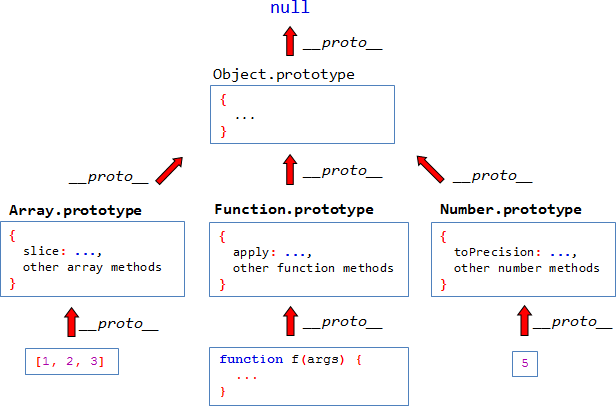
\epsfig{file=chapter1/javascript_natives.eps, width=12cm}}
\end{center}

\end{figure}%
\lthtmlfigureZ
\lthtmlcheckvsize\clearpage}

{\newpage\clearpage
\lthtmlfigureA{figure1160}%
\begin{figure}\begin{center}
\centerline{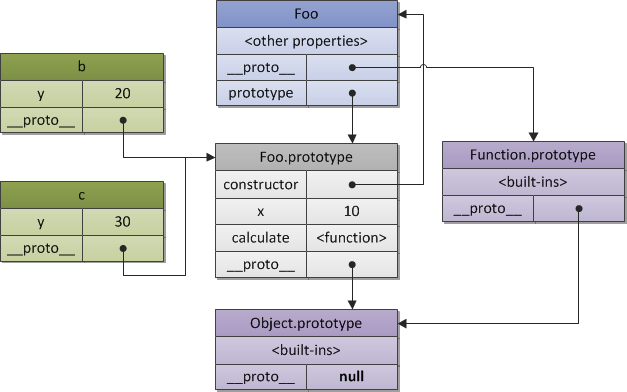
\epsfig{file=chapter1/proto_and_prototypes.eps, width=12cm}}
\end{center}

\end{figure}%
\lthtmlfigureZ
\lthtmlcheckvsize\clearpage}

\stepcounter{section}
\stepcounter{section}
\stepcounter{chapter}
\stepcounter{chapter}
\stepcounter{section}
\stepcounter{section}
\stepcounter{section}
\stepcounter{section}
\stepcounter{section}
\stepcounter{section}
\stepcounter{section}
\stepcounter{subsection}
\stepcounter{subsection}
\stepcounter{subsection}
\stepcounter{section}
\stepcounter{chapter}
\stepcounter{section}
\stepcounter{section}
\stepcounter{chapter}
\stepcounter{chapter}
\stepcounter{section}
\stepcounter{section}
\stepcounter{section}
\stepcounter{section}
\stepcounter{section}
\stepcounter{section}
\stepcounter{section}
\stepcounter{section}
\stepcounter{subsection}
\stepcounter{subsection}
\stepcounter{subsection}
\stepcounter{subsection}
\stepcounter{subsection}
\stepcounter{subsection}
\stepcounter{subsection}
\stepcounter{subsection}
\stepcounter{paragraph}
\stepcounter{paragraph}
\stepcounter{paragraph}
\stepcounter{paragraph}
\stepcounter{paragraph}
\stepcounter{section}
\stepcounter{subsection}
\stepcounter{subsection}
\stepcounter{subsection}
\stepcounter{subsection}
\stepcounter{section}
\stepcounter{chapter}
\stepcounter{chapter}
\stepcounter{chapter}
\stepcounter{chapter}
\stepcounter{chapter}
\stepcounter{chapter}
\stepcounter{chapter}
\stepcounter{chapter}
\stepcounter{chapter}
\stepcounter{chapter}
\stepcounter{chapter}
\stepcounter{chapter}
\stepcounter{chapter}
\stepcounter{section}
\stepcounter{chapter}
\stepcounter{section}
\stepcounter{section}
\stepcounter{chapter}
\stepcounter{section}
\stepcounter{chapter}
\stepcounter{section}
\stepcounter{section}
\stepcounter{section}
\stepcounter{paragraph}
\stepcounter{section}
\stepcounter{section}
\stepcounter{section}
\stepcounter{section}
\stepcounter{part}
\stepcounter{chapter}
\stepcounter{section}
\stepcounter{section}
\stepcounter{paragraph}
\stepcounter{paragraph}
\stepcounter{paragraph}
\stepcounter{section}
\stepcounter{paragraph}
\stepcounter{paragraph}
\stepcounter{paragraph}
\stepcounter{paragraph}
\stepcounter{paragraph}
\stepcounter{paragraph}
\stepcounter{section}
\stepcounter{section}
\stepcounter{paragraph}
{\newpage\clearpage
\lthtmlfigureA{figure2117}%
\begin{figure}\begin{center}
\end{center}

\end{figure}%
\lthtmlfigureZ
\lthtmlcheckvsize\clearpage}

\stepcounter{paragraph}
\stepcounter{paragraph}
\stepcounter{paragraph}
\stepcounter{paragraph}
\stepcounter{paragraph}
\stepcounter{section}
\stepcounter{section}
\stepcounter{section}
\stepcounter{paragraph}
\stepcounter{paragraph}
\stepcounter{paragraph}
\stepcounter{paragraph}
\stepcounter{section}
\stepcounter{chapter}
\stepcounter{section}
\stepcounter{paragraph}
\stepcounter{section}
\stepcounter{subsection}
\stepcounter{paragraph}
\stepcounter{paragraph}
\stepcounter{paragraph}
\stepcounter{paragraph}
\stepcounter{paragraph}
\stepcounter{paragraph}
\stepcounter{subsection}
\stepcounter{subsection}
\stepcounter{subsection}
\stepcounter{subsection}
\stepcounter{subsection}
\stepcounter{subsection}
\stepcounter{subsection}
\stepcounter{subsection}
\stepcounter{subsection}
\stepcounter{subsection}
\stepcounter{subsection}
\stepcounter{subsection}
\stepcounter{subsection}
\stepcounter{subsection}
\stepcounter{subsubsection}
{\newpage\clearpage
\lthtmlinlinemathA{tex2html_wrap_inline35551}%
$ \{a^n b^n\  /\  n \in N\}$%
\lthtmlinlinemathZ
\lthtmlcheckvsize\clearpage}

\stepcounter{subsection}
\stepcounter{subsection}
\stepcounter{subsection}
\stepcounter{subsection}
\stepcounter{subsection}
\stepcounter{subsection}
\stepcounter{subsection}
\stepcounter{subsection}
\stepcounter{subsection}
\stepcounter{subsection}
\stepcounter{subsection}
\stepcounter{subsection}
\stepcounter{chapter}
\stepcounter{section}
\stepcounter{section}
{\newpage\clearpage
\lthtmlinlinemathA{tex2html_wrap_inline35568}%
$ \backslash$%
\lthtmlinlinemathZ
\lthtmlcheckvsize\clearpage}

\stepcounter{section}
\stepcounter{section}
\stepcounter{section}
\stepcounter{section}
\stepcounter{section}
\stepcounter{section}
\stepcounter{section}
\stepcounter{section}
\stepcounter{section}
\stepcounter{section}
\stepcounter{chapter}
\stepcounter{section}
\stepcounter{paragraph}
\stepcounter{subsection}
\stepcounter{paragraph}
\stepcounter{paragraph}
\stepcounter{paragraph}
\stepcounter{paragraph}
\stepcounter{paragraph}
\stepcounter{paragraph}
\stepcounter{paragraph}
\stepcounter{paragraph}
\stepcounter{paragraph}
\stepcounter{paragraph}
\stepcounter{paragraph}
\stepcounter{paragraph}
\stepcounter{paragraph}
\stepcounter{paragraph}
{\newpage\clearpage
\lthtmlinlinemathA{tex2html_wrap_inline35632}%
$ n$%
\lthtmlinlinemathZ
\lthtmlcheckvsize\clearpage}

{\newpage\clearpage
\lthtmlinlinemathA{tex2html_wrap_inline35634}%
$ k$%
\lthtmlinlinemathZ
\lthtmlcheckvsize\clearpage}

{\newpage\clearpage
\lthtmlinlinemathA{tex2html_wrap_inline35636}%
$ n-k$%
\lthtmlinlinemathZ
\lthtmlcheckvsize\clearpage}

{\newpage\clearpage
\lthtmlinlinemathA{tex2html_wrap_inline35638}%
$ m$%
\lthtmlinlinemathZ
\lthtmlcheckvsize\clearpage}

\stepcounter{paragraph}
\stepcounter{paragraph}
\stepcounter{paragraph}
\stepcounter{paragraph}
\stepcounter{paragraph}
\stepcounter{paragraph}
{\newpage\clearpage
\lthtmlinlinemathA{tex2html_wrap_inline35650}%
$ \backslash k$%
\lthtmlinlinemathZ
\lthtmlcheckvsize\clearpage}

{\newpage\clearpage
\lthtmlinlinemathA{tex2html_wrap_inline35652}%
$ \backslash g$%
\lthtmlinlinemathZ
\lthtmlcheckvsize\clearpage}

\stepcounter{paragraph}
\stepcounter{paragraph}
\stepcounter{paragraph}
\stepcounter{paragraph}
\stepcounter{paragraph}
\stepcounter{subsection}
\stepcounter{subsection}
\stepcounter{paragraph}
\stepcounter{paragraph}
\stepcounter{paragraph}
\stepcounter{paragraph}
\stepcounter{paragraph}
\stepcounter{paragraph}
\stepcounter{paragraph}
\stepcounter{subsubsection}
\stepcounter{paragraph}
\stepcounter{paragraph}
\stepcounter{paragraph}
\stepcounter{subsection}
\stepcounter{paragraph}
\stepcounter{paragraph}
\stepcounter{paragraph}
\stepcounter{paragraph}
\stepcounter{paragraph}
\stepcounter{paragraph}
\stepcounter{paragraph}
\stepcounter{paragraph}
\stepcounter{subsection}
\stepcounter{subsection}
\stepcounter{paragraph}
\stepcounter{paragraph}
\stepcounter{section}
\stepcounter{subsection}
\stepcounter{subsection}
\stepcounter{subsection}
\stepcounter{paragraph}
\stepcounter{paragraph}
\stepcounter{paragraph}
\stepcounter{paragraph}
\stepcounter{paragraph}
\stepcounter{paragraph}
\stepcounter{paragraph}
\stepcounter{paragraph}
\stepcounter{paragraph}
\stepcounter{paragraph}
\stepcounter{paragraph}
\stepcounter{paragraph}
\stepcounter{paragraph}
\stepcounter{subsection}
\stepcounter{paragraph}
\stepcounter{paragraph}
\stepcounter{paragraph}
\stepcounter{subsection}
\stepcounter{paragraph}
\stepcounter{paragraph}
\stepcounter{paragraph}
\stepcounter{paragraph}
\stepcounter{paragraph}
\stepcounter{paragraph}
\stepcounter{subsection}
\stepcounter{paragraph}
\stepcounter{paragraph}
\stepcounter{paragraph}
\stepcounter{paragraph}
\stepcounter{paragraph}
\stepcounter{subsection}
\stepcounter{subsection}
\stepcounter{paragraph}
\stepcounter{paragraph}
\stepcounter{paragraph}
\stepcounter{paragraph}
\stepcounter{paragraph}
\stepcounter{paragraph}
\stepcounter{paragraph}
\stepcounter{subsection}
\stepcounter{paragraph}
\stepcounter{paragraph}
\stepcounter{paragraph}
\stepcounter{paragraph}
\stepcounter{paragraph}
\stepcounter{paragraph}
\stepcounter{subsection}
\stepcounter{paragraph}
\stepcounter{paragraph}
\stepcounter{paragraph}
\stepcounter{paragraph}
\stepcounter{paragraph}
\stepcounter{paragraph}
\stepcounter{subsection}
\stepcounter{paragraph}
\stepcounter{paragraph}
\stepcounter{paragraph}
\stepcounter{paragraph}
\stepcounter{paragraph}
\stepcounter{section}
\stepcounter{paragraph}
\stepcounter{paragraph}
\stepcounter{paragraph}
\stepcounter{paragraph}
\stepcounter{paragraph}
\stepcounter{paragraph}
\stepcounter{paragraph}
\stepcounter{paragraph}
\stepcounter{paragraph}
\stepcounter{paragraph}
\stepcounter{paragraph}
\stepcounter{paragraph}
\stepcounter{section}
\stepcounter{paragraph}
\stepcounter{paragraph}
\stepcounter{paragraph}
\stepcounter{paragraph}
\stepcounter{paragraph}
\stepcounter{paragraph}
\stepcounter{paragraph}
\stepcounter{section}
\stepcounter{subsection}
\stepcounter{paragraph}
\stepcounter{paragraph}
\stepcounter{subsection}
\stepcounter{subsection}
\stepcounter{subsection}
\stepcounter{paragraph}
\stepcounter{paragraph}
\stepcounter{paragraph}
\stepcounter{paragraph}
\stepcounter{paragraph}
\stepcounter{paragraph}
\stepcounter{paragraph}
\stepcounter{subsection}
\stepcounter{subsection}
\stepcounter{subsection}
\stepcounter{section}
\stepcounter{section}
\stepcounter{section}
\stepcounter{section}
\stepcounter{subsection}
\stepcounter{paragraph}
\stepcounter{paragraph}
\stepcounter{paragraph}
\stepcounter{paragraph}
\stepcounter{paragraph}
\stepcounter{subsection}
\stepcounter{paragraph}
\stepcounter{paragraph}
\stepcounter{paragraph}
\stepcounter{section}
\stepcounter{section}
\stepcounter{subsection}
\stepcounter{paragraph}
\stepcounter{paragraph}
\stepcounter{paragraph}
\stepcounter{paragraph}
\stepcounter{paragraph}
\stepcounter{paragraph}
\stepcounter{paragraph}
\stepcounter{paragraph}
\stepcounter{paragraph}
\stepcounter{subsection}
\stepcounter{subsection}
\stepcounter{paragraph}
\stepcounter{paragraph}
\stepcounter{paragraph}
\stepcounter{paragraph}
\stepcounter{paragraph}
\stepcounter{subsection}
\stepcounter{paragraph}
\stepcounter{paragraph}
\stepcounter{paragraph}
\stepcounter{paragraph}
\stepcounter{paragraph}
\stepcounter{paragraph}
\stepcounter{subsection}
\stepcounter{paragraph}
\stepcounter{paragraph}
\stepcounter{paragraph}
\stepcounter{subsection}
\stepcounter{paragraph}
\stepcounter{subsection}
\stepcounter{paragraph}
\stepcounter{paragraph}
\stepcounter{subsection}
\stepcounter{subsection}
\stepcounter{paragraph}
\stepcounter{paragraph}
\stepcounter{paragraph}
\stepcounter{paragraph}
\stepcounter{paragraph}
\stepcounter{paragraph}
\stepcounter{paragraph}
\stepcounter{paragraph}
\stepcounter{subsection}
\stepcounter{subsection}
\stepcounter{paragraph}
\stepcounter{subsection}
\stepcounter{paragraph}
\stepcounter{paragraph}
\stepcounter{subsection}
\stepcounter{subsection}
\stepcounter{subsection}
\stepcounter{subsection}
\stepcounter{subsection}
\stepcounter{subsection}
\stepcounter{paragraph}
\stepcounter{paragraph}
\stepcounter{paragraph}
\stepcounter{paragraph}
\stepcounter{paragraph}
\stepcounter{paragraph}
\stepcounter{subsection}
\stepcounter{chapter}
\stepcounter{section}
\stepcounter{section}
\stepcounter{subsection}
\stepcounter{chapter}
\stepcounter{section}
\stepcounter{paragraph}
\stepcounter{paragraph}
\stepcounter{paragraph}
\stepcounter{paragraph}
\stepcounter{subsection}
\stepcounter{subsection}
\stepcounter{section}
\stepcounter{paragraph}
\stepcounter{paragraph}
\stepcounter{paragraph}
\stepcounter{paragraph}
\stepcounter{paragraph}
\stepcounter{paragraph}
\stepcounter{paragraph}
\stepcounter{paragraph}
\stepcounter{subsection}
\stepcounter{subsection}
\stepcounter{section}
\stepcounter{paragraph}
\stepcounter{paragraph}
\stepcounter{paragraph}
\stepcounter{paragraph}
\stepcounter{paragraph}
\stepcounter{paragraph}
\stepcounter{paragraph}
\stepcounter{paragraph}
\stepcounter{subsection}
\stepcounter{subsection}
\stepcounter{subsection}
\stepcounter{subsection}
\stepcounter{subsection}
\stepcounter{subsection}
\stepcounter{section}
\stepcounter{paragraph}
\stepcounter{paragraph}
\stepcounter{paragraph}
\stepcounter{paragraph}
\stepcounter{subsection}
\stepcounter{paragraph}
\stepcounter{paragraph}
\stepcounter{paragraph}
\stepcounter{paragraph}
\stepcounter{subsubsection}
\stepcounter{subsection}
\stepcounter{subsection}
\stepcounter{section}
{\newpage\clearpage
\lthtmlinlinemathA{tex2html_wrap_inline36096}%
$ A$%
\lthtmlinlinemathZ
\lthtmlcheckvsize\clearpage}

{\newpage\clearpage
\lthtmlinlinemathA{tex2html_wrap_inline36098}%
$ A^*$%
\lthtmlinlinemathZ
\lthtmlcheckvsize\clearpage}

{\newpage\clearpage
\lthtmlinlinemathA{tex2html_wrap_inline36102}%
$ A^* = \cup_{n=0}^{\infty} A^n
$%
\lthtmlinlinemathZ
\lthtmlcheckvsize\clearpage}

{\newpage\clearpage
\lthtmlinlinemathA{tex2html_wrap_inline36104}%
$ A^0 = \{ \epsilon \}$%
\lthtmlinlinemathZ
\lthtmlcheckvsize\clearpage}

{\newpage\clearpage
\lthtmlinlinemathA{tex2html_wrap_inline36106}%
$ \epsilon$%
\lthtmlinlinemathZ
\lthtmlcheckvsize\clearpage}

{\newpage\clearpage
\lthtmlinlinemathA{tex2html_wrap_inline36115}%
$ G$%
\lthtmlinlinemathZ
\lthtmlcheckvsize\clearpage}

{\newpage\clearpage
\lthtmlinlinemathA{tex2html_wrap_inline36117}%
$ G =(\Sigma,V,P,S)$%
\lthtmlinlinemathZ
\lthtmlcheckvsize\clearpage}

{\newpage\clearpage
\lthtmlinlinemathA{tex2html_wrap_inline36119}%
$ \Sigma$%
\lthtmlinlinemathZ
\lthtmlcheckvsize\clearpage}

{\newpage\clearpage
\lthtmlinlinemathA{tex2html_wrap_inline36121}%
$ V$%
\lthtmlinlinemathZ
\lthtmlcheckvsize\clearpage}

{\newpage\clearpage
\lthtmlinlinemathA{tex2html_wrap_inline36125}%
$ V \times (V \cup \Sigma )^*$%
\lthtmlinlinemathZ
\lthtmlcheckvsize\clearpage}

{\newpage\clearpage
\lthtmlinlinemathA{tex2html_wrap_inline36127}%
$ (A, \alpha) \in P$%
\lthtmlinlinemathZ
\lthtmlcheckvsize\clearpage}

{\newpage\clearpage
\lthtmlinlinemathA{tex2html_wrap_inline36129}%
$ A \rightarrow \alpha$%
\lthtmlinlinemathZ
\lthtmlcheckvsize\clearpage}

{\newpage\clearpage
\lthtmlinlinemathA{tex2html_wrap_inline36131}%
$ P$%
\lthtmlinlinemathZ
\lthtmlcheckvsize\clearpage}

{\newpage\clearpage
\lthtmlinlinemathA{tex2html_wrap_inline36133}%
$ S$%
\lthtmlinlinemathZ
\lthtmlcheckvsize\clearpage}

{\newpage\clearpage
\lthtmlinlinemathA{tex2html_wrap_inline36144}%
$ \mu = \alpha A \beta \in (V \cup \Sigma)^*$%
\lthtmlinlinemathZ
\lthtmlcheckvsize\clearpage}

{\newpage\clearpage
\lthtmlinlinemathA{tex2html_wrap_inline36146}%
$ A \rightarrow \gamma$%
\lthtmlinlinemathZ
\lthtmlcheckvsize\clearpage}

{\newpage\clearpage
\lthtmlinlinemathA{tex2html_wrap_inline36150}%
$ \mu$%
\lthtmlinlinemathZ
\lthtmlcheckvsize\clearpage}

{\newpage\clearpage
\lthtmlinlinemathA{tex2html_wrap_inline36152}%
$ \alpha \gamma \beta$%
\lthtmlinlinemathZ
\lthtmlcheckvsize\clearpage}

{\newpage\clearpage
\lthtmlinlinemathA{tex2html_wrap_inline36154}%
$ \alpha A \beta$%
\lthtmlinlinemathZ
\lthtmlcheckvsize\clearpage}

{\newpage\clearpage
\lthtmlinlinemathA{tex2html_wrap_inline36160}%
$ \gamma$%
\lthtmlinlinemathZ
\lthtmlcheckvsize\clearpage}

{\newpage\clearpage
\lthtmlinlinemathA{tex2html_wrap_inline36166}%
$ \delta$%
\lthtmlinlinemathZ
\lthtmlcheckvsize\clearpage}

{\newpage\clearpage
\lthtmlinlinemathA{tex2html_wrap_inline36168}%
$ n-1$%
\lthtmlinlinemathZ
\lthtmlcheckvsize\clearpage}

{\newpage\clearpage
\lthtmlinlinemathA{tex2html_wrap_inline36174}%
$ \mu  \stackrel{*}{\Longrightarrow}  \delta$%
\lthtmlinlinemathZ
\lthtmlcheckvsize\clearpage}

{\newpage\clearpage
\lthtmlinlinemathA{tex2html_wrap_inline36183}%
$ L(G)$%
\lthtmlinlinemathZ
\lthtmlcheckvsize\clearpage}

{\newpage\clearpage
\lthtmlinlinemathA{tex2html_wrap_inline36187}%
$ L(G) = \{ x \in \Sigma^* : S \stackrel{*}{\Longrightarrow} x \}$%
\lthtmlinlinemathZ
\lthtmlcheckvsize\clearpage}

{\newpage\clearpage
\lthtmlinlinemathA{tex2html_wrap_inline36200}%
$ \alpha A x$%
\lthtmlinlinemathZ
\lthtmlcheckvsize\clearpage}

{\newpage\clearpage
\lthtmlinlinemathA{tex2html_wrap_inline36206}%
$ x A \alpha$%
\lthtmlinlinemathZ
\lthtmlcheckvsize\clearpage}

{\newpage\clearpage
\lthtmlinlinemathA{tex2html_wrap_inline36215}%
$ V \cup \Sigma$%
\lthtmlinlinemathZ
\lthtmlcheckvsize\clearpage}

{\newpage\clearpage
\lthtmlinlinemathA{tex2html_wrap_inline36221}%
$ X_1 \ldots X_n$%
\lthtmlinlinemathZ
\lthtmlcheckvsize\clearpage}

{\newpage\clearpage
\lthtmlinlinemathA{tex2html_wrap_inline36223}%
$ \gamma = X_1 \ldots X_n$%
\lthtmlinlinemathZ
\lthtmlcheckvsize\clearpage}

{\newpage\clearpage
\lthtmlinlinemathA{tex2html_wrap_inline36230}%
$ x \in L(G)$%
\lthtmlinlinemathZ
\lthtmlcheckvsize\clearpage}

{\newpage\clearpage
\lthtmlinlinemathA{tex2html_wrap_inline36232}%
$ x_1 \ldots x_n$%
\lthtmlinlinemathZ
\lthtmlcheckvsize\clearpage}

{\newpage\clearpage
\lthtmlinlinemathA{tex2html_wrap_inline36234}%
$ x$%
\lthtmlinlinemathZ
\lthtmlcheckvsize\clearpage}

\stepcounter{subsection}
{\newpage\clearpage
\lthtmlinlinemathA{tex2html_wrap_inline36250}%
$ \rightarrow$%
\lthtmlinlinemathZ
\lthtmlcheckvsize\clearpage}

{\newpage\clearpage
\lthtmlinlinemathA{tex2html_wrap_inline36252}%
$ |$%
\lthtmlinlinemathZ
\lthtmlcheckvsize\clearpage}

{\newpage\clearpage
\lthtmlinlinemathA{tex2html_wrap_inline36303}%
$ S =$%
\lthtmlinlinemathZ
\lthtmlcheckvsize\clearpage}

\stepcounter{section}
\stepcounter{subsection}
{\newpage\clearpage
\lthtmlinlinemathA{tex2html_wrap_inline36307}%
$ A \in V$%
\lthtmlinlinemathZ
\lthtmlcheckvsize\clearpage}

{\newpage\clearpage
\lthtmlinlinemathA{tex2html_wrap_inline36311}%
$ L_A(G) = \{ x \in \Sigma^* : A \stackrel{*}{\Longrightarrow} x \}$%
\lthtmlinlinemathZ
\lthtmlcheckvsize\clearpage}

{\newpage\clearpage
\lthtmlinlinemathA{tex2html_wrap_inline36317}%
$ L(A)$%
\lthtmlinlinemathZ
\lthtmlcheckvsize\clearpage}

{\newpage\clearpage
\lthtmlinlinemathA{tex2html_wrap_inline36323}%
$ a$%
\lthtmlinlinemathZ
\lthtmlcheckvsize\clearpage}

{\newpage\clearpage
\lthtmlinlinemathA{tex2html_wrap_inline36327}%
$ \alpha$%
\lthtmlinlinemathZ
\lthtmlcheckvsize\clearpage}

{\newpage\clearpage
\lthtmlinlinemathA{tex2html_wrap_inline36333}%
$ L_{\alpha}(G)$%
\lthtmlinlinemathZ
\lthtmlcheckvsize\clearpage}

{\newpage\clearpage
\lthtmlinlinemathA{tex2html_wrap_inline36337}%
$ \alpha = X_1 \ldots X_n$%
\lthtmlinlinemathZ
\lthtmlcheckvsize\clearpage}

{\newpage\clearpage
\lthtmlinlinemathA{tex2html_wrap_inline36339}%
$ X_i$%
\lthtmlinlinemathZ
\lthtmlcheckvsize\clearpage}

{\newpage\clearpage
\lthtmlinlinemathA{tex2html_wrap_inline36343}%
$ X_i = B$%
\lthtmlinlinemathZ
\lthtmlcheckvsize\clearpage}

{\newpage\clearpage
\lthtmlinlinemathA{tex2html_wrap_inline36383}%
$ A \rightarrow a \alpha$%
\lthtmlinlinemathZ
\lthtmlcheckvsize\clearpage}

{\newpage\clearpage
\lthtmlinlinemathA{tex2html_wrap_inline36391}%
$ FIRST(\alpha)$%
\lthtmlinlinemathZ
\lthtmlcheckvsize\clearpage}

{\newpage\clearpage
\lthtmlinlinemathA{tex2html_wrap_inline36400}%
$ \alpha \in (V \cup \Sigma)^*$%
\lthtmlinlinemathZ
\lthtmlcheckvsize\clearpage}

{\newpage\clearpage
\lthtmlinlinemathA{tex2html_wrap_inline36404}%
$ FIRST(\alpha) = \left \{ b \in \Sigma :  \alpha  \stackrel{*}{\Longrightarrow}  b \beta \right \}
\cup N(\alpha)$%
\lthtmlinlinemathZ
\lthtmlcheckvsize\clearpage}

{\newpage\clearpage
\lthtmlinlinemathA{tex2html_wrap_inline36406}%
$ N(\alpha) = \left \{ \begin{array}{ll}
                         \left \{ \epsilon \right \}& \mbox{si $\alpha \stackrel{*}{\Longrightarrow} \epsilon$} \\
                         \emptyset & \mbox{en otro caso} 
                      \end{array}
             \right. $%
\lthtmlinlinemathZ
\lthtmlcheckvsize\clearpage}

{\newpage\clearpage
\lthtmlinlinemathA{tex2html_wrap_inline36408}%
$ A \rightarrow \gamma_1 \mid \ldots \mid \gamma_n$%
\lthtmlinlinemathZ
\lthtmlcheckvsize\clearpage}

{\newpage\clearpage
\lthtmlinlinemathA{tex2html_wrap_inline36410}%
$ FIRST(\gamma_i)$%
\lthtmlinlinemathZ
\lthtmlcheckvsize\clearpage}

{\newpage\clearpage
\lthtmlinlinemathA{tex2html_wrap_inline36414}%
$ \gamma_j$%
\lthtmlinlinemathZ
\lthtmlcheckvsize\clearpage}

{\newpage\clearpage
\lthtmlinlinemathA{tex2html_wrap_inline36416}%
$ X_1 \ldots X_k$%
\lthtmlinlinemathZ
\lthtmlcheckvsize\clearpage}

{\newpage\clearpage
\lthtmlinlinemathA{tex2html_wrap_inline36418}%
$ i = 1 \ldots k$%
\lthtmlinlinemathZ
\lthtmlcheckvsize\clearpage}

\stepcounter{subsection}
\stepcounter{subsection}
{\newpage\clearpage
\lthtmlinlinemathA{tex2html_wrap_inline36447}%
$ A   \rightarrow \alpha \beta \mid \alpha \gamma$%
\lthtmlinlinemathZ
\lthtmlcheckvsize\clearpage}

{\newpage\clearpage
\lthtmlinlinemathA{tex2html_wrap_inline36452}%
$ FIRST(\beta) \cap FIRST(\gamma) = \emptyset$%
\lthtmlinlinemathZ
\lthtmlcheckvsize\clearpage}

\stepcounter{subsection}
{\newpage\clearpage
\lthtmlinlinemathA{tex2html_wrap_inline36463}%
$ \epsilon \in FIRST(\gamma)$%
\lthtmlinlinemathZ
\lthtmlcheckvsize\clearpage}

{\newpage\clearpage
\lthtmlinlinemathA{tex2html_wrap_inline36465}%
$ \gamma \stackrel{*}{\Longrightarrow} \epsilon$%
\lthtmlinlinemathZ
\lthtmlcheckvsize\clearpage}

{\newpage\clearpage
\lthtmlinlinemathA{tex2html_wrap_inline36469}%
$ S \stackrel{*}{\Longrightarrow} \beta A\  a \mu \Longrightarrow \beta \gamma\  a \mu \stackrel{*}{\Longrightarrow} \beta\  a \mu$%
\lthtmlinlinemathZ
\lthtmlcheckvsize\clearpage}

{\newpage\clearpage
\lthtmlinlinemathA{tex2html_wrap_inline36471}%
$ a \in \Sigma$%
\lthtmlinlinemathZ
\lthtmlcheckvsize\clearpage}

{\newpage\clearpage
\lthtmlinlinemathA{tex2html_wrap_inline36481}%
$ FOLLOW(A)$%
\lthtmlinlinemathZ
\lthtmlcheckvsize\clearpage}

{\newpage\clearpage
\lthtmlinlinemathA{tex2html_wrap_inline36496}%
$ FOLLOW(A) = \left \{ b \in \Sigma :  \exists\  S  \stackrel{*}{\Longrightarrow}  \alpha A b \beta \right \} \cup E(A)$%
\lthtmlinlinemathZ
\lthtmlcheckvsize\clearpage}

{\newpage\clearpage
\lthtmlinlinemathA{tex2html_wrap_inline36498}%
$ E(A) = \left \{ \begin{array}{ll}
                         \{ \$  \}& \mbox{si $S \stackrel{*}{\Longrightarrow} \alpha A$} \\
                         \emptyset & \mbox{en otro caso} 
                      \end{array}
             \right. $%
\lthtmlinlinemathZ
\lthtmlcheckvsize\clearpage}

{\newpage\clearpage
\lthtmlinlinemathA{tex2html_wrap_inline36500}%
$ \$$%
\lthtmlinlinemathZ
\lthtmlcheckvsize\clearpage}

{\newpage\clearpage
\lthtmlinlinemathA{tex2html_wrap_inline36508}%
$ \gamma_n$%
\lthtmlinlinemathZ
\lthtmlcheckvsize\clearpage}

{\newpage\clearpage
\lthtmlinlinemathA{tex2html_wrap_inline36512}%
$ \gamma_n \stackrel{*}{\Longrightarrow} \epsilon$%
\lthtmlinlinemathZ
\lthtmlcheckvsize\clearpage}

{\newpage\clearpage
\lthtmlinlinemathA{tex2html_wrap_inline36514}%
$ \gamma_n = \epsilon$%
\lthtmlinlinemathZ
\lthtmlcheckvsize\clearpage}

\stepcounter{subsection}
{\newpage\clearpage
\lthtmlinlinemathA{tex2html_wrap_inline36522}%
$ FIRST(X)$%
\lthtmlinlinemathZ
\lthtmlcheckvsize\clearpage}

{\newpage\clearpage
\lthtmlinlinemathA{tex2html_wrap_inline36526}%
$ Si\  X \in \Sigma\  entonces\  FIRST(X) = {X}$%
\lthtmlinlinemathZ
\lthtmlcheckvsize\clearpage}

{\newpage\clearpage
\lthtmlinlinemathA{tex2html_wrap_inline36528}%
$ Si\  X \rightarrow \epsilon\  entonces\  FIRST(X) =  FIRST(X) \cup \{ \epsilon \}$%
\lthtmlinlinemathZ
\lthtmlcheckvsize\clearpage}

{\newpage\clearpage
\lthtmlinlinemathA{tex2html_wrap_inline36530}%
$ Si X \in V \  y\  X \rightarrow Y_1 Y_2 \cdots Y_k \in P\  entonces$%
\lthtmlinlinemathZ
\lthtmlcheckvsize\clearpage}

{\newpage\clearpage
\lthtmlinlinemathA{tex2html_wrap_indisplay36533}%
$\displaystyle i = 1;$%
\lthtmlindisplaymathZ
\lthtmlcheckvsize\clearpage}

{\newpage\clearpage
\lthtmlinlinemathA{tex2html_wrap_indisplay36535}%
$\displaystyle hacer$%
\lthtmlindisplaymathZ
\lthtmlcheckvsize\clearpage}

{\newpage\clearpage
\lthtmlinlinemathA{tex2html_wrap_indisplay36537}%
$\displaystyle \  \ FIRST(X) = FIRST(X) \cup FIRST^*(Y_i);$%
\lthtmlindisplaymathZ
\lthtmlcheckvsize\clearpage}

{\newpage\clearpage
\lthtmlinlinemathA{tex2html_wrap_indisplay36539}%
$\displaystyle \  \ i++;$%
\lthtmlindisplaymathZ
\lthtmlcheckvsize\clearpage}

{\newpage\clearpage
\lthtmlinlinemathA{tex2html_wrap_indisplay36541}%
$\displaystyle mientras\  (i \leq k\  y\  \epsilon \in FIRST(Y_i))$%
\lthtmlindisplaymathZ
\lthtmlcheckvsize\clearpage}

{\newpage\clearpage
\lthtmlinlinemathA{tex2html_wrap_inline36547}%
$ i \geq k$%
\lthtmlinlinemathZ
\lthtmlcheckvsize\clearpage}

{\newpage\clearpage
\lthtmlinlinemathA{tex2html_wrap_inline36549}%
$ \epsilon \in FIRST(Y_k)$%
\lthtmlinlinemathZ
\lthtmlcheckvsize\clearpage}

{\newpage\clearpage
\lthtmlinlinemathA{tex2html_wrap_inline36551}%
$ FIRST^*(Y)$%
\lthtmlinlinemathZ
\lthtmlcheckvsize\clearpage}

{\newpage\clearpage
\lthtmlinlinemathA{tex2html_wrap_inline36553}%
$ FIRST(Y) - \{ \epsilon \}$%
\lthtmlinlinemathZ
\lthtmlcheckvsize\clearpage}

{\newpage\clearpage
\lthtmlinlinemathA{tex2html_wrap_inline36557}%
$ \alpha = X_1 X_2 \cdots X_n \in (V \cup \Sigma)^*$%
\lthtmlinlinemathZ
\lthtmlcheckvsize\clearpage}

{\newpage\clearpage
\lthtmlinlinemathA{tex2html_wrap_indisplay36571}%
$\displaystyle FIRST(\alpha) = \emptyset;$%
\lthtmlindisplaymathZ
\lthtmlcheckvsize\clearpage}

{\newpage\clearpage
\lthtmlinlinemathA{tex2html_wrap_indisplay36575}%
$\displaystyle \  \ FIRST(\alpha) = FIRST(\alpha) \cup FIRST^*(X_i);$%
\lthtmlindisplaymathZ
\lthtmlcheckvsize\clearpage}

{\newpage\clearpage
\lthtmlinlinemathA{tex2html_wrap_indisplay36579}%
$\displaystyle mientras\  (i \leq n\  y\  \epsilon \in FIRST(X_i))$%
\lthtmlindisplaymathZ
\lthtmlcheckvsize\clearpage}

{\newpage\clearpage
\lthtmlinlinemathA{tex2html_wrap_inline36586}%
$ FOLLOW(A)\  \forall A \in V$%
\lthtmlinlinemathZ
\lthtmlcheckvsize\clearpage}

{\newpage\clearpage
\lthtmlinlinemathA{tex2html_wrap_inline36590}%
$ FOLLOW(S) = \{\$\} $%
\lthtmlinlinemathZ
\lthtmlcheckvsize\clearpage}

{\newpage\clearpage
\lthtmlinlinemathA{tex2html_wrap_inline36594}%
$ Si\  A \rightarrow \alpha B \beta\  entonces$%
\lthtmlinlinemathZ
\lthtmlcheckvsize\clearpage}

{\newpage\clearpage
\lthtmlinlinemathA{tex2html_wrap_indisplay36596}%
$\displaystyle FOLLOW(B) =  FOLLOW(B) \cup (FIRST(\beta) - \{\epsilon\})$%
\lthtmlindisplaymathZ
\lthtmlcheckvsize\clearpage}

{\newpage\clearpage
\lthtmlinlinemathA{tex2html_wrap_inline36598}%
$ Si\  A \rightarrow \alpha B\  o\  A \rightarrow \alpha B \beta\  y\  \epsilon \in FIRST(\beta)\   entonces$%
\lthtmlinlinemathZ
\lthtmlcheckvsize\clearpage}

{\newpage\clearpage
\lthtmlinlinemathA{tex2html_wrap_indisplay36600}%
$\displaystyle FOLLOW(B) = FOLLOW(B) \cup FOLLOW(A)$%
\lthtmlindisplaymathZ
\lthtmlcheckvsize\clearpage}

\stepcounter{subsection}
\stepcounter{subsection}
{\newpage\clearpage
\lthtmlinlinemathA{tex2html_wrap_inline36622}%
$ |\  \epsilon$%
\lthtmlinlinemathZ
\lthtmlcheckvsize\clearpage}

\stepcounter{subsection}
\stepcounter{subsection}
{\newpage\clearpage
\lthtmlinlinemathA{tex2html_wrap_inline36653}%
$ A \rightarrow \beta$%
\lthtmlinlinemathZ
\lthtmlcheckvsize\clearpage}

{\newpage\clearpage
\lthtmlinlinemathA{tex2html_wrap_inline36657}%
$ FIRST(\alpha) \cap FIRST(\beta) = \emptyset$%
\lthtmlinlinemathZ
\lthtmlcheckvsize\clearpage}

{\newpage\clearpage
\lthtmlinlinemathA{tex2html_wrap_inline36659}%
$ \epsilon \in FIRST(\alpha)$%
\lthtmlinlinemathZ
\lthtmlcheckvsize\clearpage}

{\newpage\clearpage
\lthtmlinlinemathA{tex2html_wrap_inline36661}%
$ FIRST(\alpha) \cap FOLLOW(A) = \emptyset$%
\lthtmlinlinemathZ
\lthtmlcheckvsize\clearpage}

\stepcounter{subsection}
{\newpage\clearpage
\lthtmlinlinemathA{tex2html_wrap_inline36674}%
$ FIRST(\alpha) = \emptyset$%
\lthtmlinlinemathZ
\lthtmlcheckvsize\clearpage}

{\newpage\clearpage
\lthtmlinlinemathA{tex2html_wrap_inline36678}%
$ FOLLOW(A) = \emptyset$%
\lthtmlinlinemathZ
\lthtmlcheckvsize\clearpage}

\stepcounter{subsection}
\stepcounter{subsection}
\stepcounter{subsection}
\stepcounter{paragraph}
\stepcounter{paragraph}
\stepcounter{paragraph}
\stepcounter{paragraph}
{\newpage\clearpage
\lthtmlinlinemathA{tex2html_wrap_inline36738}%
$ (terminal, atributo)$%
\lthtmlinlinemathZ
\lthtmlcheckvsize\clearpage}

\stepcounter{paragraph}
\stepcounter{paragraph}
\stepcounter{paragraph}
\stepcounter{paragraph}
\stepcounter{section}
{\newpage\clearpage
\lthtmlinlinemathA{tex2html_wrap_inline36754}%
$ A \rightarrow \alpha \beta $%
\lthtmlinlinemathZ
\lthtmlcheckvsize\clearpage}

{\newpage\clearpage
\lthtmlinlinemathA{tex2html_wrap_inline36756}%
$ A \rightarrow \alpha \{ action \} \beta $%
\lthtmlinlinemathZ
\lthtmlcheckvsize\clearpage}

{\newpage\clearpage
\lthtmlinlinemathA{tex2html_wrap_inline36758}%
$ \{ action \}$%
\lthtmlinlinemathZ
\lthtmlcheckvsize\clearpage}

{\newpage\clearpage
\lthtmlinlinemathA{tex2html_wrap_inline36762}%
$ \beta$%
\lthtmlinlinemathZ
\lthtmlcheckvsize\clearpage}

{\newpage\clearpage
\lthtmlinlinemathA{tex2html_wrap_inline36764}%
$ expr   \rightarrow expr_1  -  NUM$%
\lthtmlinlinemathZ
\lthtmlcheckvsize\clearpage}

{\newpage\clearpage
\lthtmlinlinemathA{tex2html_wrap_inline36766}%
$ expr   \rightarrow NUM$%
\lthtmlinlinemathZ
\lthtmlcheckvsize\clearpage}

{\newpage\clearpage
\lthtmlinlinemathA{tex2html_wrap_inline36772}%
$ NUM$%
\lthtmlinlinemathZ
\lthtmlcheckvsize\clearpage}

{\newpage\clearpage
\lthtmlinlinemathA{tex2html_wrap_inline36774}%
$ expr$%
\lthtmlinlinemathZ
\lthtmlcheckvsize\clearpage}

{\newpage\clearpage
\lthtmlinlinemathA{tex2html_wrap_inline36791}%
$ decl   \rightarrow type$%
\lthtmlinlinemathZ
\lthtmlcheckvsize\clearpage}

{\newpage\clearpage
\lthtmlinlinemathA{tex2html_wrap_inline36793}%
$ list$%
\lthtmlinlinemathZ
\lthtmlcheckvsize\clearpage}

{\newpage\clearpage
\lthtmlinlinemathA{tex2html_wrap_inline36795}%
$ type   \rightarrow INT$%
\lthtmlinlinemathZ
\lthtmlcheckvsize\clearpage}

{\newpage\clearpage
\lthtmlinlinemathA{tex2html_wrap_inline36797}%
$ type   \rightarrow STRING$%
\lthtmlinlinemathZ
\lthtmlcheckvsize\clearpage}

{\newpage\clearpage
\lthtmlinlinemathA{tex2html_wrap_inline36799}%
$ list   \rightarrow ID$%
\lthtmlinlinemathZ
\lthtmlcheckvsize\clearpage}

{\newpage\clearpage
\lthtmlinlinemathA{tex2html_wrap_inline36801}%
$ list_1$%
\lthtmlinlinemathZ
\lthtmlcheckvsize\clearpage}

\stepcounter{section}
{\newpage\clearpage
\lthtmlinlinemathA{tex2html_wrap_inline36833}%
$ A \stackrel{*}{\Longrightarrow} A \alpha$%
\lthtmlinlinemathZ
\lthtmlcheckvsize\clearpage}

{\newpage\clearpage
\lthtmlinlinemathA{tex2html_wrap_inline36835}%
$ A \rightarrow A \alpha$%
\lthtmlinlinemathZ
\lthtmlcheckvsize\clearpage}

\stepcounter{subsection}
{\newpage\clearpage
\lthtmlinlinemathA{tex2html_wrap_inline36844}%
$ |\  \beta$%
\lthtmlinlinemathZ
\lthtmlcheckvsize\clearpage}

{\newpage\clearpage
\lthtmlinlinemathA{tex2html_wrap_inline36848}%
$ \alpha, \beta \in (V \cup \Sigma)^*$%
\lthtmlinlinemathZ
\lthtmlcheckvsize\clearpage}

{\newpage\clearpage
\lthtmlinlinemathA{tex2html_wrap_inline36852}%
$ A   \rightarrow \beta R$%
\lthtmlinlinemathZ
\lthtmlcheckvsize\clearpage}

{\newpage\clearpage
\lthtmlinlinemathA{tex2html_wrap_inline36854}%
$ R   \rightarrow  \alpha R$%
\lthtmlinlinemathZ
\lthtmlcheckvsize\clearpage}

{\newpage\clearpage
\lthtmlinlinemathA{tex2html_wrap_inline36874}%
$ expr   \rightarrow expr  -  NUM$%
\lthtmlinlinemathZ
\lthtmlcheckvsize\clearpage}

{\newpage\clearpage
\lthtmlinlinemathA{tex2html_wrap_inline36885}%
$ expr   \rightarrow NUM - expr_1$%
\lthtmlinlinemathZ
\lthtmlcheckvsize\clearpage}

{\newpage\clearpage
\lthtmlinlinemathA{tex2html_wrap_inline36898}%
$ e   \rightarrow\  NUM\  r$%
\lthtmlinlinemathZ
\lthtmlcheckvsize\clearpage}

{\newpage\clearpage
\lthtmlinlinemathA{tex2html_wrap_inline36900}%
$ r   \rightarrow - e$%
\lthtmlinlinemathZ
\lthtmlcheckvsize\clearpage}

{\newpage\clearpage
\lthtmlinlinemathA{tex2html_wrap_inline36902}%
$ r   \rightarrow \epsilon$%
\lthtmlinlinemathZ
\lthtmlcheckvsize\clearpage}

\stepcounter{subsection}
{\newpage\clearpage
\lthtmlinlinemathA{tex2html_wrap_inline36925}%
$ A   \rightarrow A \beta$%
\lthtmlinlinemathZ
\lthtmlcheckvsize\clearpage}

{\newpage\clearpage
\lthtmlinlinemathA{tex2html_wrap_inline36935}%
$ \gamma \beta \alpha$%
\lthtmlinlinemathZ
\lthtmlcheckvsize\clearpage}

{\newpage\clearpage
\lthtmlinlinemathA{tex2html_wrap_inline36939}%
$ R$%
\lthtmlinlinemathZ
\lthtmlcheckvsize\clearpage}

{\newpage\clearpage
\lthtmlinlinemathA{tex2html_wrap_inline36941}%
$ R   \rightarrow \beta$%
\lthtmlinlinemathZ
\lthtmlcheckvsize\clearpage}

{\newpage\clearpage
\lthtmlinlinemathA{tex2html_wrap_inline36945}%
$ R   \rightarrow \alpha$%
\lthtmlinlinemathZ
\lthtmlcheckvsize\clearpage}

{\newpage\clearpage
\lthtmlinlinemathA{tex2html_wrap_inline36949}%
$ R   \rightarrow \epsilon$%
\lthtmlinlinemathZ
\lthtmlcheckvsize\clearpage}

{\newpage\clearpage
\lthtmlinlinemathA{tex2html_wrap_inline36963}%
$ r$%
\lthtmlinlinemathZ
\lthtmlcheckvsize\clearpage}

{\newpage\clearpage
\lthtmlinlinemathA{tex2html_wrap_inline36971}%
$ r   \rightarrow - NUM$%
\lthtmlinlinemathZ
\lthtmlcheckvsize\clearpage}

{\newpage\clearpage
\lthtmlinlinemathA{tex2html_wrap_inline36973}%
$ r_1$%
\lthtmlinlinemathZ
\lthtmlcheckvsize\clearpage}

\stepcounter{subsection}
\stepcounter{subsection}
\stepcounter{subsection}
{\newpage\clearpage
\lthtmlinlinemathA{tex2html_wrap_inline36990}%
$ A^s$%
\lthtmlinlinemathZ
\lthtmlcheckvsize\clearpage}

{\newpage\clearpage
\lthtmlinlinemathA{tex2html_wrap_inline36992}%
$ A   \rightarrow A_1 X_1 X_2 X_3$%
\lthtmlinlinemathZ
\lthtmlcheckvsize\clearpage}

{\newpage\clearpage
\lthtmlinlinemathA{tex2html_wrap_inline36994}%
$ \{ A^s = f_X(A^s_1, X_1^s, X_2^s, X_3^s) \}$%
\lthtmlinlinemathZ
\lthtmlcheckvsize\clearpage}

{\newpage\clearpage
\lthtmlinlinemathA{tex2html_wrap_inline36996}%
$ A   \rightarrow A_1 Y_1 Y_2 Y_3$%
\lthtmlinlinemathZ
\lthtmlcheckvsize\clearpage}

{\newpage\clearpage
\lthtmlinlinemathA{tex2html_wrap_inline36998}%
$ \{ A^s = f_Y(A^s_1, Y_1^s, Y_2^s, Y_3^s) \}$%
\lthtmlinlinemathZ
\lthtmlcheckvsize\clearpage}

{\newpage\clearpage
\lthtmlinlinemathA{tex2html_wrap_inline37000}%
$ A   \rightarrow Z_1 Z_2 Z_3$%
\lthtmlinlinemathZ
\lthtmlcheckvsize\clearpage}

{\newpage\clearpage
\lthtmlinlinemathA{tex2html_wrap_inline37002}%
$ \{ A^s = f_Z(Z_1^s, Z_2^s, Z_3^s) \}$%
\lthtmlinlinemathZ
\lthtmlcheckvsize\clearpage}

{\newpage\clearpage
\lthtmlinlinemathA{tex2html_wrap_inline37010}%
$ f_X, f_Y$%
\lthtmlinlinemathZ
\lthtmlcheckvsize\clearpage}

{\newpage\clearpage
\lthtmlinlinemathA{tex2html_wrap_inline37012}%
$ f_Z$%
\lthtmlinlinemathZ
\lthtmlcheckvsize\clearpage}

\stepcounter{subsection}
{\newpage\clearpage
\lthtmlinlinemathA{tex2html_wrap_inline37059}%
$ \rightarrow \epsilon$%
\lthtmlinlinemathZ
\lthtmlcheckvsize\clearpage}

\stepcounter{section}
\stepcounter{subsection}
{\newpage\clearpage
\lthtmlinlinemathA{tex2html_wrap_inline37137}%
$ (\Sigma, \rho)$%
\lthtmlinlinemathZ
\lthtmlcheckvsize\clearpage}

{\newpage\clearpage
\lthtmlinlinemathA{tex2html_wrap_inline37141}%
$ \rho$%
\lthtmlinlinemathZ
\lthtmlcheckvsize\clearpage}

{\newpage\clearpage
\lthtmlinlinemathA{tex2html_wrap_inline37143}%
$ \rho: \Sigma \rightarrow \mathds{N}_0$%
\lthtmlinlinemathZ
\lthtmlcheckvsize\clearpage}

{\newpage\clearpage
\lthtmlinlinemathA{tex2html_wrap_inline37145}%
$ \Sigma_k = \{ a \in \Sigma :\  \rho(a) = k \}$%
\lthtmlinlinemathZ
\lthtmlcheckvsize\clearpage}

{\newpage\clearpage
\lthtmlinlinemathA{tex2html_wrap_inline37147}%
$ B(\Sigma)$%
\lthtmlinlinemathZ
\lthtmlcheckvsize\clearpage}

{\newpage\clearpage
\lthtmlinlinemathA{tex2html_wrap_inline37153}%
$ a \in  \Sigma_0$%
\lthtmlinlinemathZ
\lthtmlcheckvsize\clearpage}

{\newpage\clearpage
\lthtmlinlinemathA{tex2html_wrap_inline37155}%
$ a \in B(\Sigma)$%
\lthtmlinlinemathZ
\lthtmlcheckvsize\clearpage}

{\newpage\clearpage
\lthtmlinlinemathA{tex2html_wrap_inline37157}%
$ b_1, \ldots , b_k \in B(\Sigma)$%
\lthtmlinlinemathZ
\lthtmlcheckvsize\clearpage}

{\newpage\clearpage
\lthtmlinlinemathA{tex2html_wrap_inline37159}%
$ f \in \Sigma_k$%
\lthtmlinlinemathZ
\lthtmlcheckvsize\clearpage}

{\newpage\clearpage
\lthtmlinlinemathA{tex2html_wrap_inline37163}%
$ f(b_1, \ldots , b_k) \in B(\Sigma)$%
\lthtmlinlinemathZ
\lthtmlcheckvsize\clearpage}

{\newpage\clearpage
\lthtmlinlinemathA{tex2html_wrap_inline37172}%
$ \Sigma = \{A, CONS, NIL \}$%
\lthtmlinlinemathZ
\lthtmlcheckvsize\clearpage}

{\newpage\clearpage
\lthtmlinlinemathA{tex2html_wrap_inline37174}%
$ \rho(A) = \rho(NIL) = 0, \rho(CONS) = 2$%
\lthtmlinlinemathZ
\lthtmlcheckvsize\clearpage}

{\newpage\clearpage
\lthtmlinlinemathA{tex2html_wrap_inline37176}%
$ B(\Sigma) = \{ A, NIL, CONS(A,NIL), CONS(NIL, A), CONS(A, A), CONS(NIL,NIL), \ldots \}$%
\lthtmlinlinemathZ
\lthtmlcheckvsize\clearpage}

{\newpage\clearpage
\lthtmlinlinemathA{tex2html_wrap_inline37183}%
$ \Sigma = \{ID, NUM, LEFTVALUE, STR, PLUS, TIMES, ASSIGN, PRINT \}$%
\lthtmlinlinemathZ
\lthtmlcheckvsize\clearpage}

{\newpage\clearpage
\lthtmlinlinemathA{tex2html_wrap_inline37185}%
$ \rho(ID) = \rho(NUM) = \rho(LEFTVALUE) = \rho(STR) = 0$%
\lthtmlinlinemathZ
\lthtmlcheckvsize\clearpage}

{\newpage\clearpage
\lthtmlinlinemathA{tex2html_wrap_inline37187}%
$ \rho(PRINT) = 1$%
\lthtmlinlinemathZ
\lthtmlcheckvsize\clearpage}

{\newpage\clearpage
\lthtmlinlinemathA{tex2html_wrap_inline37189}%
$ \rho(PLUS) = \rho(TIMES) = \rho(ASSIGN) = 2$%
\lthtmlinlinemathZ
\lthtmlcheckvsize\clearpage}

{\newpage\clearpage
\lthtmlinlinemathA{tex2html_wrap_inline37197}%
$ ASSIGN(NUM, PRINT(ID))$%
\lthtmlinlinemathZ
\lthtmlcheckvsize\clearpage}

{\newpage\clearpage
\lthtmlinlinemathA{tex2html_wrap_inline37206}%
$ ((\Sigma, \rho), N, P, S)$%
\lthtmlinlinemathZ
\lthtmlcheckvsize\clearpage}

{\newpage\clearpage
\lthtmlinlinemathA{tex2html_wrap_inline37210}%
$ \rho: \Sigma \rightarrow \mathds{N}$%
\lthtmlinlinemathZ
\lthtmlcheckvsize\clearpage}

{\newpage\clearpage
\lthtmlinlinemathA{tex2html_wrap_inline37212}%
$ N$%
\lthtmlinlinemathZ
\lthtmlcheckvsize\clearpage}

{\newpage\clearpage
\lthtmlinlinemathA{tex2html_wrap_inline37216}%
$ X \rightarrow s$%
\lthtmlinlinemathZ
\lthtmlcheckvsize\clearpage}

{\newpage\clearpage
\lthtmlinlinemathA{tex2html_wrap_inline37218}%
$ X \in N$%
\lthtmlinlinemathZ
\lthtmlcheckvsize\clearpage}

{\newpage\clearpage
\lthtmlinlinemathA{tex2html_wrap_inline37220}%
$ s \in B(\Sigma \cup N)$%
\lthtmlinlinemathZ
\lthtmlcheckvsize\clearpage}

{\newpage\clearpage
\lthtmlinlinemathA{tex2html_wrap_inline37222}%
$ S \in N$%
\lthtmlinlinemathZ
\lthtmlcheckvsize\clearpage}

{\newpage\clearpage
\lthtmlinlinemathA{tex2html_wrap_inline37229}%
$ (\Sigma, N, P, S)$%
\lthtmlinlinemathZ
\lthtmlcheckvsize\clearpage}

{\newpage\clearpage
\lthtmlinlinemathA{tex2html_wrap_inline37231}%
$ t \in B(\Sigma \cup N)$%
\lthtmlinlinemathZ
\lthtmlcheckvsize\clearpage}

{\newpage\clearpage
\lthtmlinlinemathA{tex2html_wrap_inline37233}%
$ (X_1, \ldots X_k)$%
\lthtmlinlinemathZ
\lthtmlcheckvsize\clearpage}

{\newpage\clearpage
\lthtmlinlinemathA{tex2html_wrap_inline37235}%
$ j$%
\lthtmlinlinemathZ
\lthtmlcheckvsize\clearpage}

{\newpage\clearpage
\lthtmlinlinemathA{tex2html_wrap_inline37237}%
$ t$%
\lthtmlinlinemathZ
\lthtmlcheckvsize\clearpage}

{\newpage\clearpage
\lthtmlinlinemathA{tex2html_wrap_inline37239}%
$ X_j \in N$%
\lthtmlinlinemathZ
\lthtmlcheckvsize\clearpage}

{\newpage\clearpage
\lthtmlinlinemathA{tex2html_wrap_inline37241}%
$ p = X \rightarrow s$%
\lthtmlinlinemathZ
\lthtmlcheckvsize\clearpage}

{\newpage\clearpage
\lthtmlinlinemathA{tex2html_wrap_inline37243}%
$ s$%
\lthtmlinlinemathZ
\lthtmlcheckvsize\clearpage}

{\newpage\clearpage
\lthtmlinlinemathA{tex2html_wrap_inline37245}%
$ (X_1, \ldots X_n)$%
\lthtmlinlinemathZ
\lthtmlcheckvsize\clearpage}

{\newpage\clearpage
\lthtmlinlinemathA{tex2html_wrap_inline37247}%
$ p$%
\lthtmlinlinemathZ
\lthtmlcheckvsize\clearpage}

{\newpage\clearpage
\lthtmlinlinemathA{tex2html_wrap_inline37249}%
$ (X_1, \ldots X_n) \rightarrow X$%
\lthtmlinlinemathZ
\lthtmlcheckvsize\clearpage}

{\newpage\clearpage
\lthtmlinlinemathA{tex2html_wrap_inline37262}%
$ X_i \rightarrow s_i \in P$%
\lthtmlinlinemathZ
\lthtmlcheckvsize\clearpage}

{\newpage\clearpage
\lthtmlinlinemathA{tex2html_wrap_inline37264}%
$ i$%
\lthtmlinlinemathZ
\lthtmlcheckvsize\clearpage}

{\newpage\clearpage
\lthtmlinlinemathA{tex2html_wrap_inline37268}%
$ t'$%
\lthtmlinlinemathZ
\lthtmlcheckvsize\clearpage}

{\newpage\clearpage
\lthtmlinlinemathA{tex2html_wrap_inline37272}%
$ s_i$%
\lthtmlinlinemathZ
\lthtmlcheckvsize\clearpage}

{\newpage\clearpage
\lthtmlinlinemathA{tex2html_wrap_inline37274}%
$ t \Longrightarrow t'$%
\lthtmlinlinemathZ
\lthtmlcheckvsize\clearpage}

{\newpage\clearpage
\lthtmlinlinemathA{tex2html_wrap_inline37276}%
$ t' = t\{X_i/s_i\}$%
\lthtmlinlinemathZ
\lthtmlcheckvsize\clearpage}

{\newpage\clearpage
\lthtmlinlinemathA{tex2html_wrap_inline37278}%
$ t \stackrel{0}{\Longrightarrow} t$%
\lthtmlinlinemathZ
\lthtmlcheckvsize\clearpage}

{\newpage\clearpage
\lthtmlinlinemathA{tex2html_wrap_inline37286}%
$ t \stackrel{n}{\Longrightarrow} t'$%
\lthtmlinlinemathZ
\lthtmlcheckvsize\clearpage}

{\newpage\clearpage
\lthtmlinlinemathA{tex2html_wrap_inline37290}%
$ t''$%
\lthtmlinlinemathZ
\lthtmlcheckvsize\clearpage}

{\newpage\clearpage
\lthtmlinlinemathA{tex2html_wrap_inline37300}%
$ t \stackrel{*}{\Longrightarrow} t'$%
\lthtmlinlinemathZ
\lthtmlcheckvsize\clearpage}

{\newpage\clearpage
\lthtmlinlinemathA{tex2html_wrap_inline37307}%
$ G = (\Sigma, N, P, S)$%
\lthtmlinlinemathZ
\lthtmlcheckvsize\clearpage}

{\newpage\clearpage
\lthtmlinlinemathA{tex2html_wrap_inline37309}%
$ L(G) = \{ t \in B(\Sigma): \exists S \stackrel{*}{\Longrightarrow} t \}$%
\lthtmlinlinemathZ
\lthtmlcheckvsize\clearpage}

{\newpage\clearpage
\lthtmlinlinemathA{tex2html_wrap_inline37322}%
$ V = \{ E, L \}$%
\lthtmlinlinemathZ
\lthtmlcheckvsize\clearpage}

{\newpage\clearpage
\lthtmlinlinemathA{tex2html_wrap_inline37326}%
$ P_1 = \{ L \rightarrow NIL, L \rightarrow CONS(E,L),E \rightarrow a \}$%
\lthtmlinlinemathZ
\lthtmlcheckvsize\clearpage}

{\newpage\clearpage
\lthtmlinlinemathA{tex2html_wrap_inline37328}%
$ L \rightarrow CONS(E,L)$%
\lthtmlinlinemathZ
\lthtmlcheckvsize\clearpage}

{\newpage\clearpage
\lthtmlinlinemathA{tex2html_wrap_inline37330}%
$ (E,L) \rightarrow L$%
\lthtmlinlinemathZ
\lthtmlcheckvsize\clearpage}

{\newpage\clearpage
\lthtmlinlinemathA{tex2html_wrap_inline37340}%
$ L(G) = \{ NIL, CONS(A, NIL), CONS(A, CONS(A,NIL)), \ldots \}$%
\lthtmlinlinemathZ
\lthtmlcheckvsize\clearpage}

{\newpage\clearpage
\lthtmlinlinemathA{tex2html_wrap_inline37347}%
$ CONS(A, CONS(A,NIL))$%
\lthtmlinlinemathZ
\lthtmlcheckvsize\clearpage}

{\newpage\clearpage
\lthtmlinlinemathA{tex2html_wrap_inline37349}%
$ CONS(E, CONS(A, CONS(E,L)))$%
\lthtmlinlinemathZ
\lthtmlcheckvsize\clearpage}

{\newpage\clearpage
\lthtmlinlinemathA{tex2html_wrap_inline37366}%
$ V = \{ st, expr \}$%
\lthtmlinlinemathZ
\lthtmlcheckvsize\clearpage}

{\newpage\clearpage
\lthtmlinlinemathA{tex2html_wrap_inline37373}%
$ P =$%
\lthtmlinlinemathZ
\lthtmlcheckvsize\clearpage}

{\newpage\clearpage
\lthtmlinlinemathA{tex2html_wrap_inline37375}%
$ \{$%
\lthtmlinlinemathZ
\lthtmlcheckvsize\clearpage}

{\newpage\clearpage
\lthtmlinlinemathA{tex2html_wrap_inline37377}%
$ st$%
\lthtmlinlinemathZ
\lthtmlcheckvsize\clearpage}

{\newpage\clearpage
\lthtmlinlinemathA{tex2html_wrap_inline37379}%
$ \rightarrow ASSIGN(LEFTVALUE, expr)$%
\lthtmlinlinemathZ
\lthtmlcheckvsize\clearpage}

{\newpage\clearpage
\lthtmlinlinemathA{tex2html_wrap_inline37383}%
$ \rightarrow PRINT(expr)$%
\lthtmlinlinemathZ
\lthtmlcheckvsize\clearpage}

{\newpage\clearpage
\lthtmlinlinemathA{tex2html_wrap_inline37387}%
$ \rightarrow PLUS(expr, expr)$%
\lthtmlinlinemathZ
\lthtmlcheckvsize\clearpage}

{\newpage\clearpage
\lthtmlinlinemathA{tex2html_wrap_inline37391}%
$ \rightarrow TIMES(expr, expr)$%
\lthtmlinlinemathZ
\lthtmlcheckvsize\clearpage}

{\newpage\clearpage
\lthtmlinlinemathA{tex2html_wrap_inline37395}%
$ \rightarrow NUM$%
\lthtmlinlinemathZ
\lthtmlcheckvsize\clearpage}

{\newpage\clearpage
\lthtmlinlinemathA{tex2html_wrap_inline37399}%
$ \rightarrow ID$%
\lthtmlinlinemathZ
\lthtmlcheckvsize\clearpage}

{\newpage\clearpage
\lthtmlinlinemathA{tex2html_wrap_inline37403}%
$ \rightarrow STR$%
\lthtmlinlinemathZ
\lthtmlcheckvsize\clearpage}

{\newpage\clearpage
\lthtmlinlinemathA{tex2html_wrap_inline37405}%
$ \}$%
\lthtmlinlinemathZ
\lthtmlcheckvsize\clearpage}

{\newpage\clearpage
\lthtmlinlinemathA{tex2html_wrap_inline37436}%
$ ASSIGN$%
\lthtmlinlinemathZ
\lthtmlcheckvsize\clearpage}

{\newpage\clearpage
\lthtmlinlinemathA{tex2html_wrap_inline37438}%
$ ($%
\lthtmlinlinemathZ
\lthtmlcheckvsize\clearpage}

{\newpage\clearpage
\lthtmlinlinemathA{tex2html_wrap_inline37440}%
$ LEFTVALUE$%
\lthtmlinlinemathZ
\lthtmlcheckvsize\clearpage}

{\newpage\clearpage
\lthtmlinlinemathA{tex2html_wrap_inline37442}%
$ PLUS$%
\lthtmlinlinemathZ
\lthtmlcheckvsize\clearpage}

{\newpage\clearpage
\lthtmlinlinemathA{tex2html_wrap_inline37446}%
$ ID$%
\lthtmlinlinemathZ
\lthtmlcheckvsize\clearpage}

{\newpage\clearpage
\lthtmlinlinemathA{tex2html_wrap_inline37448}%
$ TIMES$%
\lthtmlinlinemathZ
\lthtmlcheckvsize\clearpage}

{\newpage\clearpage
\lthtmlinlinemathA{tex2html_wrap_inline37456}%
$ )$%
\lthtmlinlinemathZ
\lthtmlcheckvsize\clearpage}

{\newpage\clearpage
\lthtmlinlinemathA{tex2html_wrap_inline37509}%
$ T = (\Omega, N, R, U)$%
\lthtmlinlinemathZ
\lthtmlcheckvsize\clearpage}

{\newpage\clearpage
\lthtmlinlinemathA{tex2html_wrap_inline37511}%
$ L(T)$%
\lthtmlinlinemathZ
\lthtmlcheckvsize\clearpage}

{\newpage\clearpage
\lthtmlinlinemathA{tex2html_wrap_inline37517}%
$ \Omega$%
\lthtmlinlinemathZ
\lthtmlcheckvsize\clearpage}

{\newpage\clearpage
\lthtmlinlinemathA{tex2html_wrap_inline37529}%
$ t \in B(\Sigma)$%
\lthtmlinlinemathZ
\lthtmlcheckvsize\clearpage}

{\newpage\clearpage
\lthtmlinlinemathA{tex2html_wrap_inline37533}%
$ t/\epsilon = t$%
\lthtmlinlinemathZ
\lthtmlcheckvsize\clearpage}

{\newpage\clearpage
\lthtmlinlinemathA{tex2html_wrap_inline37535}%
$ t = a(t_1, \ldots t_k)$%
\lthtmlinlinemathZ
\lthtmlcheckvsize\clearpage}

{\newpage\clearpage
\lthtmlinlinemathA{tex2html_wrap_inline37537}%
$ j \in \{ 1 \ldots k \}$%
\lthtmlinlinemathZ
\lthtmlcheckvsize\clearpage}

{\newpage\clearpage
\lthtmlinlinemathA{tex2html_wrap_inline37541}%
$ t/j.n$%
\lthtmlinlinemathZ
\lthtmlcheckvsize\clearpage}

{\newpage\clearpage
\lthtmlinlinemathA{tex2html_wrap_inline37549}%
$ t/j.n = t_j/n$%
\lthtmlinlinemathZ
\lthtmlcheckvsize\clearpage}

{\newpage\clearpage
\lthtmlinlinemathA{tex2html_wrap_inline37556}%
$ t = ASSIGN$%
\lthtmlinlinemathZ
\lthtmlcheckvsize\clearpage}

{\newpage\clearpage
\lthtmlinlinemathA{tex2html_wrap_inline37622}%
$ t/\epsilon$%
\lthtmlinlinemathZ
\lthtmlcheckvsize\clearpage}

{\newpage\clearpage
\lthtmlinlinemathA{tex2html_wrap_inline37624}%
$ t/2\ldotp2\ldotp1$%
\lthtmlinlinemathZ
\lthtmlcheckvsize\clearpage}

{\newpage\clearpage
\lthtmlinlinemathA{tex2html_wrap_inline37626}%
$ t/2\ldotp1$%
\lthtmlinlinemathZ
\lthtmlcheckvsize\clearpage}

{\newpage\clearpage
\lthtmlinlinemathA{tex2html_wrap_inline37628}%
$ t/2\ldotp1\ldotp2$%
\lthtmlinlinemathZ
\lthtmlcheckvsize\clearpage}

\stepcounter{subsection}
{\newpage\clearpage
\lthtmlinlinemathA{tex2html_wrap_inline37636}%
$ prog$%
\lthtmlinlinemathZ
\lthtmlcheckvsize\clearpage}

{\newpage\clearpage
\lthtmlinlinemathA{tex2html_wrap_inline37638}%
$ \rightarrow PROGRAM(decls, sts)$%
\lthtmlinlinemathZ
\lthtmlcheckvsize\clearpage}

{\newpage\clearpage
\lthtmlinlinemathA{tex2html_wrap_inline37640}%
$ decls$%
\lthtmlinlinemathZ
\lthtmlcheckvsize\clearpage}

{\newpage\clearpage
\lthtmlinlinemathA{tex2html_wrap_inline37644}%
$ decl$%
\lthtmlinlinemathZ
\lthtmlcheckvsize\clearpage}

{\newpage\clearpage
\lthtmlinlinemathA{tex2html_wrap_inline37646}%
$ sts$%
\lthtmlinlinemathZ
\lthtmlcheckvsize\clearpage}

{\newpage\clearpage
\lthtmlinlinemathA{tex2html_wrap_inline37654}%
$ \rightarrow INT(idlist)$%
\lthtmlinlinemathZ
\lthtmlcheckvsize\clearpage}

{\newpage\clearpage
\lthtmlinlinemathA{tex2html_wrap_inline37658}%
$ \rightarrow STRING(idlist)$%
\lthtmlinlinemathZ
\lthtmlcheckvsize\clearpage}

{\newpage\clearpage
\lthtmlinlinemathA{tex2html_wrap_inline37660}%
$ idlist$%
\lthtmlinlinemathZ
\lthtmlcheckvsize\clearpage}

{\newpage\clearpage
\lthtmlinlinemathA{tex2html_wrap_inline37664}%
$ SIMPLEID$%
\lthtmlinlinemathZ
\lthtmlcheckvsize\clearpage}

{\newpage\clearpage
\lthtmlinlinemathA{tex2html_wrap_inline37739}%
$ PRINT$%
\lthtmlinlinemathZ
\lthtmlcheckvsize\clearpage}

{\newpage\clearpage
\lthtmlinlinemathA{tex2html_wrap_inline37743}%
$ e   \rightarrow\  e_1 + f$%
\lthtmlinlinemathZ
\lthtmlcheckvsize\clearpage}

{\newpage\clearpage
\lthtmlinlinemathA{tex2html_wrap_inline37745}%
$ f   \rightarrow NUM$%
\lthtmlinlinemathZ
\lthtmlcheckvsize\clearpage}

{\newpage\clearpage
\lthtmlinlinemathA{tex2html_wrap_inline37747}%
$ f   \rightarrow ID$%
\lthtmlinlinemathZ
\lthtmlcheckvsize\clearpage}

\stepcounter{subsection}
{\newpage\clearpage
\lthtmlinlinemathA{tex2html_wrap_inline37758}%
$ \rightarrow list\  decl$%
\lthtmlinlinemathZ
\lthtmlcheckvsize\clearpage}

{\newpage\clearpage
\lthtmlinlinemathA{tex2html_wrap_inline37766}%
$ \rightarrow list\  st$%
\lthtmlinlinemathZ
\lthtmlcheckvsize\clearpage}

{\newpage\clearpage
\lthtmlinlinemathA{tex2html_wrap_inline37774}%
$ \rightarrow list\  SIMPLEID$%
\lthtmlinlinemathZ
\lthtmlcheckvsize\clearpage}

\stepcounter{subsection}
{\newpage\clearpage
\lthtmlinlinemathA{tex2html_wrap_inline37789}%
$ INT$%
\lthtmlinlinemathZ
\lthtmlcheckvsize\clearpage}

{\newpage\clearpage
\lthtmlinlinemathA{tex2html_wrap_inline37791}%
$ STRING$%
\lthtmlinlinemathZ
\lthtmlcheckvsize\clearpage}

\stepcounter{subsection}
\stepcounter{section}
\stepcounter{subsection}
\stepcounter{subsection}
{\newpage\clearpage
\lthtmlinlinemathA{tex2html_wrap_inline38043}%
$ SYMTABLE$%
\lthtmlinlinemathZ
\lthtmlcheckvsize\clearpage}

{\newpage\clearpage
\lthtmlinlinemathA{tex2html_wrap_inline38045}%
$ BLOCK$%
\lthtmlinlinemathZ
\lthtmlcheckvsize\clearpage}

\stepcounter{section}
\stepcounter{subsection}
\stepcounter{section}
{\newpage\clearpage
\lthtmlinlinemathA{tex2html_wrap_inline38050}%
$ (p, e, action)$%
\lthtmlinlinemathZ
\lthtmlcheckvsize\clearpage}

{\newpage\clearpage
\lthtmlinlinemathA{tex2html_wrap_inline38054}%
$ e$%
\lthtmlinlinemathZ
\lthtmlcheckvsize\clearpage}

{\newpage\clearpage
\lthtmlinlinemathA{tex2html_wrap_inline38058}%
$ action$%
\lthtmlinlinemathZ
\lthtmlcheckvsize\clearpage}

{\newpage\clearpage
\lthtmlinlinemathA{tex2html_wrap_inline38062}%
$ p \Longrightarrow e$%
\lthtmlinlinemathZ
\lthtmlcheckvsize\clearpage}

{\newpage\clearpage
\lthtmlinlinemathA{tex2html_wrap_inline38064}%
$ PLUS(NUM_1, NUM_2) \Longrightarrow NUM_3$%
\lthtmlinlinemathZ
\lthtmlcheckvsize\clearpage}

{\newpage\clearpage
\lthtmlinlinemathA{tex2html_wrap_inline38066}%
$ PLUS(NUM, NUM)$%
\lthtmlinlinemathZ
\lthtmlcheckvsize\clearpage}

{\newpage\clearpage
\lthtmlinlinemathA{tex2html_wrap_inline38072}%
$ ASSIGN(LEFTVALUE, x)\  and$%
\lthtmlinlinemathZ
\lthtmlcheckvsize\clearpage}

{\newpage\clearpage
\lthtmlinlinemathA{tex2html_wrap_inline38074}%
$ \Longrightarrow NIL$%
\lthtmlinlinemathZ
\lthtmlcheckvsize\clearpage}

{\newpage\clearpage
\lthtmlinlinemathA{tex2html_wrap_inline38078}%
$ S_1$%
\lthtmlinlinemathZ
\lthtmlcheckvsize\clearpage}

{\newpage\clearpage
\lthtmlinlinemathA{tex2html_wrap_inline38080}%
$ S_2$%
\lthtmlinlinemathZ
\lthtmlcheckvsize\clearpage}

{\newpage\clearpage
\lthtmlinlinemathA{tex2html_wrap_inline38082}%
$ IFELSE(NUM, S_1, S_2)$%
\lthtmlinlinemathZ
\lthtmlcheckvsize\clearpage}

{\newpage\clearpage
\lthtmlinlinemathA{tex2html_wrap_inline38084}%
$ \Longrightarrow S_1$%
\lthtmlinlinemathZ
\lthtmlcheckvsize\clearpage}

{\newpage\clearpage
\lthtmlinlinemathA{tex2html_wrap_inline38088}%
$ \Longrightarrow S_2$%
\lthtmlinlinemathZ
\lthtmlcheckvsize\clearpage}

{\newpage\clearpage
\lthtmlinlinemathA{tex2html_wrap_inline38090}%
$ ASSIGN(LEFTVALUE, x)$%
\lthtmlinlinemathZ
\lthtmlcheckvsize\clearpage}

{\newpage\clearpage
\lthtmlinlinemathA{tex2html_wrap_inline38103}%
$ V =\{ x_1, x_2, \ldots \}$%
\lthtmlinlinemathZ
\lthtmlcheckvsize\clearpage}

{\newpage\clearpage
\lthtmlinlinemathA{tex2html_wrap_inline38105}%
$ \rho(x) = 0\  \forall x \in V$%
\lthtmlinlinemathZ
\lthtmlcheckvsize\clearpage}

{\newpage\clearpage
\lthtmlinlinemathA{tex2html_wrap_inline38107}%
$ B(V \cup \Sigma)$%
\lthtmlinlinemathZ
\lthtmlcheckvsize\clearpage}

{\newpage\clearpage
\lthtmlinlinemathA{tex2html_wrap_inline38121}%
$ (x_1, \ldots x_k)$%
\lthtmlinlinemathZ
\lthtmlcheckvsize\clearpage}

{\newpage\clearpage
\lthtmlinlinemathA{tex2html_wrap_inline38123}%
$ x_1, \ldots x_k$%
\lthtmlinlinemathZ
\lthtmlcheckvsize\clearpage}

{\newpage\clearpage
\lthtmlinlinemathA{tex2html_wrap_inline38134}%
$ V = \{ x \}$%
\lthtmlinlinemathZ
\lthtmlcheckvsize\clearpage}

{\newpage\clearpage
\lthtmlinlinemathA{tex2html_wrap_inline38138}%
$ x, CONS(A, x), CONS(A, CONS(x, NIL)), \ldots \}$%
\lthtmlinlinemathZ
\lthtmlcheckvsize\clearpage}

{\newpage\clearpage
\lthtmlinlinemathA{tex2html_wrap_inline38140}%
$ CONS(x, CONS(x, NIL))$%
\lthtmlinlinemathZ
\lthtmlcheckvsize\clearpage}

{\newpage\clearpage
\lthtmlinlinemathA{tex2html_wrap_inline38144}%
$ t/1$%
\lthtmlinlinemathZ
\lthtmlcheckvsize\clearpage}

{\newpage\clearpage
\lthtmlinlinemathA{tex2html_wrap_inline38155}%
$ S \rightarrow S_1(a, S, b)$%
\lthtmlinlinemathZ
\lthtmlcheckvsize\clearpage}

{\newpage\clearpage
\lthtmlinlinemathA{tex2html_wrap_inline38157}%
$ S \rightarrow S_2(NIL)$%
\lthtmlinlinemathZ
\lthtmlcheckvsize\clearpage}

{\newpage\clearpage
\lthtmlinlinemathA{tex2html_wrap_inline38159}%
$ S \rightarrow aSb$%
\lthtmlinlinemathZ
\lthtmlcheckvsize\clearpage}

{\newpage\clearpage
\lthtmlinlinemathA{tex2html_wrap_inline38165}%
$ S_1(a, X(NIL), b)$%
\lthtmlinlinemathZ
\lthtmlcheckvsize\clearpage}

{\newpage\clearpage
\lthtmlinlinemathA{tex2html_wrap_inline38167}%
$ \{X, Y\}$%
\lthtmlinlinemathZ
\lthtmlcheckvsize\clearpage}

{\newpage\clearpage
\lthtmlinlinemathA{tex2html_wrap_inline38169}%
$ S_1(X, Y, a)$%
\lthtmlinlinemathZ
\lthtmlcheckvsize\clearpage}

{\newpage\clearpage
\lthtmlinlinemathA{tex2html_wrap_inline38171}%
$ S_1(X, Y, Y)$%
\lthtmlinlinemathZ
\lthtmlcheckvsize\clearpage}

{\newpage\clearpage
\lthtmlinlinemathA{tex2html_wrap_inline38178}%
$ x, y, PLUS(x, y), ASSIGN(x, TIMES(y,ID)), PRINT(y) \ldots$%
\lthtmlinlinemathZ
\lthtmlcheckvsize\clearpage}

{\newpage\clearpage
\lthtmlinlinemathA{tex2html_wrap_inline38180}%
$ V = \{ x, y \}$%
\lthtmlinlinemathZ
\lthtmlcheckvsize\clearpage}

{\newpage\clearpage
\lthtmlinlinemathA{tex2html_wrap_inline38182}%
$ ASSIGN(x, TIMES(y,ID))$%
\lthtmlinlinemathZ
\lthtmlcheckvsize\clearpage}

{\newpage\clearpage
\lthtmlinlinemathA{tex2html_wrap_inline38184}%
$ (x, y)$%
\lthtmlinlinemathZ
\lthtmlcheckvsize\clearpage}

{\newpage\clearpage
\lthtmlinlinemathA{tex2html_wrap_inline38191}%
$ \theta$%
\lthtmlinlinemathZ
\lthtmlcheckvsize\clearpage}

{\newpage\clearpage
\lthtmlinlinemathA{tex2html_wrap_inline38193}%
$ \theta: V \rightarrow B(V \cup \Sigma)$%
\lthtmlinlinemathZ
\lthtmlcheckvsize\clearpage}

{\newpage\clearpage
\lthtmlinlinemathA{tex2html_wrap_inline38195}%
$ \theta : B(V \cup \Sigma) \rightarrow B(V \cup \Sigma)$%
\lthtmlinlinemathZ
\lthtmlcheckvsize\clearpage}

{\newpage\clearpage
\lthtmlinlinemathA{tex2html_wrap_inline38197}%
$ t \theta = \left \{ \begin{array}{ll}
                         x \theta & \mbox{si $t = x \in V$}\\
                         a(t_1  \theta, \ldots, t_k \theta) & \mbox{si $t = a(t_1, \ldots, t_k)$} 
                      \end{array}
             \right. $%
\lthtmlinlinemathZ
\lthtmlcheckvsize\clearpage}

{\newpage\clearpage
\lthtmlinlinemathA{tex2html_wrap_inline38203}%
$ t \theta$%
\lthtmlinlinemathZ
\lthtmlcheckvsize\clearpage}

{\newpage\clearpage
\lthtmlinlinemathA{tex2html_wrap_inline38205}%
$ t \theta = t\{x_1/x_1 \theta, \ldots x_k/x_k \theta\}$%
\lthtmlinlinemathZ
\lthtmlcheckvsize\clearpage}

{\newpage\clearpage
\lthtmlinlinemathA{tex2html_wrap_inline38216}%
$ \theta = \{x/A, y/CONS(A, NIL)\}$%
\lthtmlinlinemathZ
\lthtmlcheckvsize\clearpage}

{\newpage\clearpage
\lthtmlinlinemathA{tex2html_wrap_inline38218}%
$ CONS(x, y)$%
\lthtmlinlinemathZ
\lthtmlcheckvsize\clearpage}

{\newpage\clearpage
\lthtmlinlinemathA{tex2html_wrap_inline38222}%
$ CONS(x, y)\theta = CONS(x\theta, y\theta) = CONS(A, CONS(A, NIL))$%
\lthtmlinlinemathZ
\lthtmlcheckvsize\clearpage}

{\newpage\clearpage
\lthtmlinlinemathA{tex2html_wrap_inline38229}%
$ \theta = \{x/PLUS(NUM, x), y/TIMES(ID, NUM)\}$%
\lthtmlinlinemathZ
\lthtmlcheckvsize\clearpage}

{\newpage\clearpage
\lthtmlinlinemathA{tex2html_wrap_inline38231}%
$ PLUS(x, y)$%
\lthtmlinlinemathZ
\lthtmlcheckvsize\clearpage}

{\newpage\clearpage
\lthtmlinlinemathA{tex2html_wrap_inline38233}%
$ PLUS(PLUS(NUM,x), TIMES(ID, NUM))$%
\lthtmlinlinemathZ
\lthtmlcheckvsize\clearpage}

{\newpage\clearpage
\lthtmlinlinemathA{tex2html_wrap_inline38235}%
$ PLUS(x, y)\theta = PLUS(x\theta, y\theta) = PLUS(PLUS(NUM,x), TIMES(ID, NUM))$%
\lthtmlinlinemathZ
\lthtmlcheckvsize\clearpage}

{\newpage\clearpage
\lthtmlinlinemathA{tex2html_wrap_inline38242}%
$ \tau \in B(V \cup \Sigma)$%
\lthtmlinlinemathZ
\lthtmlcheckvsize\clearpage}

{\newpage\clearpage
\lthtmlinlinemathA{tex2html_wrap_inline38248}%
$ \tau$%
\lthtmlinlinemathZ
\lthtmlcheckvsize\clearpage}

{\newpage\clearpage
\lthtmlinlinemathA{tex2html_wrap_inline38252}%
$ t_1, \ldots t_k \in B(\Sigma)$%
\lthtmlinlinemathZ
\lthtmlcheckvsize\clearpage}

{\newpage\clearpage
\lthtmlinlinemathA{tex2html_wrap_inline38254}%
$ t = \tau \{x_1/t_1, \ldots x_k/t_k\}$%
\lthtmlinlinemathZ
\lthtmlcheckvsize\clearpage}

{\newpage\clearpage
\lthtmlinlinemathA{tex2html_wrap_inline38258}%
$ \{x_1/t_1, \ldots x_k/t_k\}$%
\lthtmlinlinemathZ
\lthtmlcheckvsize\clearpage}

{\newpage\clearpage
\lthtmlinlinemathA{tex2html_wrap_inline38265}%
$ \tau = CONS(x, NIL)$%
\lthtmlinlinemathZ
\lthtmlcheckvsize\clearpage}

{\newpage\clearpage
\lthtmlinlinemathA{tex2html_wrap_inline38267}%
$ t = CONS(CONS(A,NIL),NIL)$%
\lthtmlinlinemathZ
\lthtmlcheckvsize\clearpage}

{\newpage\clearpage
\lthtmlinlinemathA{tex2html_wrap_inline38269}%
$ t \ldotp 1$%
\lthtmlinlinemathZ
\lthtmlcheckvsize\clearpage}

{\newpage\clearpage
\lthtmlinlinemathA{tex2html_wrap_inline38271}%
$ t\{x/CONS(A,NIL)\}$%
\lthtmlinlinemathZ
\lthtmlcheckvsize\clearpage}

{\newpage\clearpage
\lthtmlinlinemathA{tex2html_wrap_inline38273}%
$ t \ldotp 1 \{x/A\}$%
\lthtmlinlinemathZ
\lthtmlcheckvsize\clearpage}

{\newpage\clearpage
\lthtmlinlinemathA{tex2html_wrap_inline38275}%
$ t = \tau \{x/CONS(A,NIL)\}$%
\lthtmlinlinemathZ
\lthtmlcheckvsize\clearpage}

{\newpage\clearpage
\lthtmlinlinemathA{tex2html_wrap_inline38277}%
$ t \ldotp 1 = \tau \{x/A\}$%
\lthtmlinlinemathZ
\lthtmlcheckvsize\clearpage}

{\newpage\clearpage
\lthtmlinlinemathA{tex2html_wrap_inline38284}%
$ \tau = PLUS(x, y)$%
\lthtmlinlinemathZ
\lthtmlcheckvsize\clearpage}

{\newpage\clearpage
\lthtmlinlinemathA{tex2html_wrap_inline38286}%
$ t = TIMES(PLUS(NUM, NUM), TIMES(ID, ID))$%
\lthtmlinlinemathZ
\lthtmlcheckvsize\clearpage}

{\newpage\clearpage
\lthtmlinlinemathA{tex2html_wrap_inline38292}%
$ \{x/t_1, y/t_2\}$%
\lthtmlinlinemathZ
\lthtmlcheckvsize\clearpage}

{\newpage\clearpage
\lthtmlinlinemathA{tex2html_wrap_inline38300}%
$ t = TIMES(PLUS(NUM, NUM), TIMES(ID, ID)) = \tau\{x/t_1, y/t_2\} =
PLUS(x, y)\{x/t_1, y/t_2\}$%
\lthtmlinlinemathZ
\lthtmlcheckvsize\clearpage}

\stepcounter{subsection}
{\newpage\clearpage
\lthtmlinlinemathA{tex2html_wrap_inline38307}%
$ PLUS(NUM, x)$%
\lthtmlinlinemathZ
\lthtmlcheckvsize\clearpage}

{\newpage\clearpage
\lthtmlinlinemathA{tex2html_wrap_inline38309}%
$ \wedge$%
\lthtmlinlinemathZ
\lthtmlcheckvsize\clearpage}

{\newpage\clearpage
\lthtmlinlinemathA{tex2html_wrap_inline38311}%
$ \Longrightarrow x$%
\lthtmlinlinemathZ
\lthtmlcheckvsize\clearpage}

{\newpage\clearpage
\lthtmlinlinemathA{tex2html_wrap_inline38313}%
$ PLUS(x, NUM)$%
\lthtmlinlinemathZ
\lthtmlcheckvsize\clearpage}

{\newpage\clearpage
\lthtmlinlinemathA{tex2html_wrap_inline38319}%
$ TIMES(NUM, x)$%
\lthtmlinlinemathZ
\lthtmlcheckvsize\clearpage}

{\newpage\clearpage
\lthtmlinlinemathA{tex2html_wrap_inline38325}%
$ TIMES(x, NUM)$%
\lthtmlinlinemathZ
\lthtmlcheckvsize\clearpage}

\stepcounter{section}
{\newpage\clearpage
\lthtmlinlinemathA{tex2html_wrap_inline38344}%
$ texto\  fuente \rightarrow arbol$%
\lthtmlinlinemathZ
\lthtmlcheckvsize\clearpage}

{\newpage\clearpage
\lthtmlinlinemathA{tex2html_wrap_inline38346}%
$ arbol \rightarrow texto\  objeto$%
\lthtmlinlinemathZ
\lthtmlcheckvsize\clearpage}

\stepcounter{subsection}
\stepcounter{section}
\stepcounter{section}
{\newpage\clearpage
\lthtmlinlinemathA{tex2html_wrap_inline38353}%
$ R_0 \ldots R_{k-1}$%
\lthtmlinlinemathZ
\lthtmlcheckvsize\clearpage}

{\newpage\clearpage
\lthtmlinlinemathA{tex2html_wrap_inline38355}%
$ R_i = M_a$%
\lthtmlinlinemathZ
\lthtmlcheckvsize\clearpage}

{\newpage\clearpage
\lthtmlinlinemathA{tex2html_wrap_inline38357}%
$ R_i = c$%
\lthtmlinlinemathZ
\lthtmlcheckvsize\clearpage}

{\newpage\clearpage
\lthtmlinlinemathA{tex2html_wrap_inline38359}%
$ M_a = R_i$%
\lthtmlinlinemathZ
\lthtmlcheckvsize\clearpage}

{\newpage\clearpage
\lthtmlinlinemathA{tex2html_wrap_inline38361}%
$ R_i += R_j$%
\lthtmlinlinemathZ
\lthtmlcheckvsize\clearpage}

{\newpage\clearpage
\lthtmlinlinemathA{tex2html_wrap_inline38363}%
$ R_i += M_a$%
\lthtmlinlinemathZ
\lthtmlcheckvsize\clearpage}

{\newpage\clearpage
\lthtmlinlinemathA{tex2html_wrap_inline38365}%
$ R_i += c$%
\lthtmlinlinemathZ
\lthtmlcheckvsize\clearpage}

{\newpage\clearpage
\lthtmlinlinemathA{tex2html_wrap_inline38381}%
$ OP(t_1, t_2)$%
\lthtmlinlinemathZ
\lthtmlcheckvsize\clearpage}

{\newpage\clearpage
\lthtmlinlinemathA{tex2html_wrap_inline38383}%
$ t_1$%
\lthtmlinlinemathZ
\lthtmlcheckvsize\clearpage}

{\newpage\clearpage
\lthtmlinlinemathA{tex2html_wrap_inline38387}%
$ t_2$%
\lthtmlinlinemathZ
\lthtmlcheckvsize\clearpage}

{\newpage\clearpage
\lthtmlinlinemathA{tex2html_wrap_inline38389}%
$ r_2$%
\lthtmlinlinemathZ
\lthtmlcheckvsize\clearpage}

{\newpage\clearpage
\lthtmlinlinemathA{tex2html_wrap_inline38391}%
$ r_1 < r_2 \le k$%
\lthtmlinlinemathZ
\lthtmlcheckvsize\clearpage}

{\newpage\clearpage
\lthtmlinlinemathA{tex2html_wrap_inline38397}%
$ r_2 = k$%
\lthtmlinlinemathZ
\lthtmlcheckvsize\clearpage}

{\newpage\clearpage
\lthtmlinlinemathA{tex2html_wrap_inline38405}%
$ r_2 - 1$%
\lthtmlinlinemathZ
\lthtmlcheckvsize\clearpage}

{\newpage\clearpage
\lthtmlinlinemathA{tex2html_wrap_inline38407}%
$ r_2 - 1 \ge r_1$%
\lthtmlinlinemathZ
\lthtmlcheckvsize\clearpage}

{\newpage\clearpage
\lthtmlinlinemathA{tex2html_wrap_inline38411}%
$ r_1 \neq r_2$%
\lthtmlinlinemathZ
\lthtmlcheckvsize\clearpage}

{\newpage\clearpage
\lthtmlinlinemathA{tex2html_wrap_inline38413}%
$ \max\{r_1, r_2\}$%
\lthtmlinlinemathZ
\lthtmlcheckvsize\clearpage}

{\newpage\clearpage
\lthtmlinlinemathA{tex2html_wrap_inline38415}%
$ r_1 + 1$%
\lthtmlinlinemathZ
\lthtmlcheckvsize\clearpage}

{\newpage\clearpage
\lthtmlinlinemathA{tex2html_wrap_inline38417}%
$ PLUS(a,b)$%
\lthtmlinlinemathZ
\lthtmlcheckvsize\clearpage}

{\newpage\clearpage
\lthtmlinlinemathA{tex2html_wrap_inline38419}%
$ b$%
\lthtmlinlinemathZ
\lthtmlcheckvsize\clearpage}

{\newpage\clearpage
\lthtmlinlinemathA{tex2html_wrap_inline38427}%
$ r_t$%
\lthtmlinlinemathZ
\lthtmlcheckvsize\clearpage}

{\newpage\clearpage
\lthtmlinlinemathA{tex2html_wrap_inline38431}%
$ r_t =  \left \{ \begin{array}{ll}
               \max\{r_1, r_2\} & \mbox{si $r_1 \neq r_2$}\\
               r_1 + 1 & \mbox{si $r_1 = r_2$} 
           \end{array}
        \right .$%
\lthtmlinlinemathZ
\lthtmlcheckvsize\clearpage}

{\newpage\clearpage
\lthtmlinlinemathA{tex2html_wrap_inline38439}%
$ \min \{r_1, r_2 \} < k$%
\lthtmlinlinemathZ
\lthtmlcheckvsize\clearpage}

{\newpage\clearpage
\lthtmlinlinemathA{tex2html_wrap_inline38441}%
$ \min \{r_1, r_2 \} \ge k$%
\lthtmlinlinemathZ
\lthtmlcheckvsize\clearpage}

\stepcounter{subsection}
{\newpage\clearpage
\lthtmlinlinemathA{tex2html_wrap_inline38462}%
$ PLUS(ID, t)$%
\lthtmlinlinemathZ
\lthtmlcheckvsize\clearpage}

{\newpage\clearpage
\lthtmlinlinemathA{tex2html_wrap_inline38464}%
$ \{ r_t \ge 1 \}$%
\lthtmlinlinemathZ
\lthtmlcheckvsize\clearpage}

{\newpage\clearpage
\lthtmlinlinemathA{tex2html_wrap_inline38472}%
$ \{ r_t \ge 1 \} \Longrightarrow PLUS(t, ID)$%
\lthtmlinlinemathZ
\lthtmlcheckvsize\clearpage}

{\newpage\clearpage
\lthtmlinlinemathA{tex2html_wrap_inline38474}%
$ \max \{2, r_t \}$%
\lthtmlinlinemathZ
\lthtmlcheckvsize\clearpage}

\stepcounter{section}
\stepcounter{subsection}
{\newpage\clearpage
\lthtmlinlinemathA{tex2html_wrap_inline38480}%
$ 2^n$%
\lthtmlinlinemathZ
\lthtmlcheckvsize\clearpage}

{\newpage\clearpage
\lthtmlinlinemathA{tex2html_wrap_inline38482}%
$ t = TIMES(TIMES(a,2),3)$%
\lthtmlinlinemathZ
\lthtmlcheckvsize\clearpage}

\stepcounter{chapter}
\stepcounter{section}
\stepcounter{subsection}
{\newpage\clearpage
\lthtmlinlinemathA{tex2html_wrap_inline38702}%

% latex2html id marker 38702
$ S = program$%
\lthtmlinlinemathZ
\lthtmlcheckvsize\clearpage}

\stepcounter{section}
\stepcounter{paragraph}
\stepcounter{paragraph}
\stepcounter{paragraph}
\stepcounter{paragraph}
\stepcounter{paragraph}
\stepcounter{paragraph}
\stepcounter{subsection}
\stepcounter{subsection}
\stepcounter{section}
\stepcounter{paragraph}
\stepcounter{paragraph}
\stepcounter{paragraph}
\stepcounter{paragraph}
\stepcounter{paragraph}
\stepcounter{paragraph}
\stepcounter{paragraph}
\stepcounter{paragraph}
\stepcounter{subsection}
\stepcounter{section}
{\newpage\clearpage
\lthtmlinlinemathA{tex2html_wrap_inline38724}%
$ FSD$%
\lthtmlinlinemathZ
\lthtmlcheckvsize\clearpage}

{\newpage\clearpage
\lthtmlinlinemathA{tex2html_wrap_inline38735}%
$ FSD = \left \{ \alpha \in (\Sigma \cup V)* : \exists S \begin{array}{c} *\\\Longrightarrow \\{\scriptstyle RM} \end{array} \alpha \right \}$%
\lthtmlinlinemathZ
\lthtmlcheckvsize\clearpage}

{\newpage\clearpage
\lthtmlinlinemathA{tex2html_wrap_inline38747}%
$ S \stackrel{*}{\Longrightarrow} y A z \Longrightarrow y w z = x$%
\lthtmlinlinemathZ
\lthtmlcheckvsize\clearpage}

{\newpage\clearpage
\lthtmlinlinemathA{tex2html_wrap_inline38749}%
$ A \rightarrow w$%
\lthtmlinlinemathZ
\lthtmlcheckvsize\clearpage}

{\newpage\clearpage
\lthtmlinlinemathA{tex2html_wrap_inline38753}%
$ \beta \alpha w$%
\lthtmlinlinemathZ
\lthtmlcheckvsize\clearpage}

{\newpage\clearpage
\lthtmlinlinemathA{tex2html_wrap_inline38759}%
$ S \stackrel{*}{\Longrightarrow} \beta A w \Longrightarrow \beta \alpha w$%
\lthtmlinlinemathZ
\lthtmlcheckvsize\clearpage}

{\newpage\clearpage
\lthtmlinlinemathA{tex2html_wrap_inline38768}%
$ \alpha = \beta \gamma x$%
\lthtmlinlinemathZ
\lthtmlcheckvsize\clearpage}

{\newpage\clearpage
\lthtmlinlinemathA{tex2html_wrap_inline38770}%
$ x \in \Sigma^*$%
\lthtmlinlinemathZ
\lthtmlcheckvsize\clearpage}

{\newpage\clearpage
\lthtmlinlinemathA{tex2html_wrap_inline38776}%
$ S \begin{array}{c} *\\\Longrightarrow  \\{\scriptstyle RM} \end{array} \beta B x \Longrightarrow \beta \gamma x = \alpha$%
\lthtmlinlinemathZ
\lthtmlcheckvsize\clearpage}

{\newpage\clearpage
\lthtmlinlinemathA{tex2html_wrap_inline38778}%
$ handle(\alpha) = (B \rightarrow \gamma, \beta \gamma)$%
\lthtmlinlinemathZ
\lthtmlcheckvsize\clearpage}

{\newpage\clearpage
\lthtmlinlinemathA{tex2html_wrap_inline38780}%
$ handle$%
\lthtmlinlinemathZ
\lthtmlcheckvsize\clearpage}

{\newpage\clearpage
\lthtmlinlinemathA{tex2html_wrap_inline38782}%
$ handle_1(\alpha) = B \rightarrow \gamma$%
\lthtmlinlinemathZ
\lthtmlcheckvsize\clearpage}

{\newpage\clearpage
\lthtmlinlinemathA{tex2html_wrap_inline38784}%
$ handle_2(\alpha) =  \beta \gamma$%
\lthtmlinlinemathZ
\lthtmlcheckvsize\clearpage}

{\newpage\clearpage
\lthtmlinlinemathA{tex2html_wrap_inline38786}%
$ \beta \gamma$%
\lthtmlinlinemathZ
\lthtmlcheckvsize\clearpage}

{\newpage\clearpage
\lthtmlinlinemathA{tex2html_wrap_inline38793}%
$ PV = \left \{ \delta \in (\Sigma \cup V)* :  \exists S \begin{array}{c} *\\\Longrightarrow \\{\scriptstyle RM} \end{array} \alpha = \beta \gamma x \mbox{ y }\delta\  es\  un\  prefijo\  de\   handle_2(\alpha) = \beta \gamma \right \}$%
\lthtmlinlinemathZ
\lthtmlcheckvsize\clearpage}

{\newpage\clearpage
\lthtmlinlinemathA{tex2html_wrap_inline38795}%
$ handle_2(\alpha)) =  \beta \gamma$%
\lthtmlinlinemathZ
\lthtmlcheckvsize\clearpage}

{\newpage\clearpage
\lthtmlinlinemathA{tex2html_wrap_inline38799}%
$ \alpha \in FSD$%
\lthtmlinlinemathZ
\lthtmlcheckvsize\clearpage}

{\newpage\clearpage
\lthtmlinlinemathA{tex2html_wrap_inline38801}%
$ PV$%
\lthtmlinlinemathZ
\lthtmlcheckvsize\clearpage}

{\newpage\clearpage
\lthtmlinlinemathA{tex2html_wrap_inline38820}%
$ (E \rightarrow E + E, 2)$%
\lthtmlinlinemathZ
\lthtmlcheckvsize\clearpage}

{\newpage\clearpage
\lthtmlinlinemathA{tex2html_wrap_inline38822}%
$ Q =  \left \{ (A \rightarrow \alpha, n) :  A \rightarrow \alpha \in P,\  n \le |\alpha| \right \}$%
\lthtmlinlinemathZ
\lthtmlcheckvsize\clearpage}

{\newpage\clearpage
\lthtmlinlinemathA{tex2html_wrap_inline38824}%
$ \mid \alpha \mid$%
\lthtmlinlinemathZ
\lthtmlcheckvsize\clearpage}

{\newpage\clearpage
\lthtmlinlinemathA{tex2html_wrap_inline38828}%
$ (A \rightarrow \alpha, n)$%
\lthtmlinlinemathZ
\lthtmlcheckvsize\clearpage}

{\newpage\clearpage
\lthtmlinlinemathA{tex2html_wrap_inline38830}%
$ A \rightarrow \beta _\uparrow \gamma$%
\lthtmlinlinemathZ
\lthtmlcheckvsize\clearpage}

{\newpage\clearpage
\lthtmlinlinemathA{tex2html_wrap_inline38832}%
$ = \alpha$%
\lthtmlinlinemathZ
\lthtmlcheckvsize\clearpage}

{\newpage\clearpage
\lthtmlinlinemathA{tex2html_wrap_inline38834}%
$ n = \mid \beta \mid$%
\lthtmlinlinemathZ
\lthtmlcheckvsize\clearpage}

{\newpage\clearpage
\lthtmlinlinemathA{tex2html_wrap_inline38836}%
$ \delta(A \rightarrow \alpha _\uparrow X \beta, X) = A \rightarrow \alpha X _\uparrow \beta\  \forall X \in  V \cup \Sigma$%
\lthtmlinlinemathZ
\lthtmlcheckvsize\clearpage}

{\newpage\clearpage
\lthtmlinlinemathA{tex2html_wrap_inline38838}%
$ \delta(A \rightarrow \alpha _\uparrow B \beta, \epsilon) = B \rightarrow 
_\uparrow \gamma\   \forall B \rightarrow \gamma \in  P$%
\lthtmlinlinemathZ
\lthtmlcheckvsize\clearpage}

{\newpage\clearpage
\lthtmlinlinemathA{tex2html_wrap_inline38840}%
$ S' \rightarrow S$%
\lthtmlinlinemathZ
\lthtmlcheckvsize\clearpage}

{\newpage\clearpage
\lthtmlinlinemathA{tex2html_wrap_inline38844}%
$ S' \rightarrow _\uparrow S$%
\lthtmlinlinemathZ
\lthtmlcheckvsize\clearpage}

{\newpage\clearpage
\lthtmlinlinemathA{tex2html_wrap_inline38846}%
$ LR(0)$%
\lthtmlinlinemathZ
\lthtmlcheckvsize\clearpage}

{\newpage\clearpage
\lthtmlinlinemathA{tex2html_wrap_inline38848}%
$ LR(0)-items$%
\lthtmlinlinemathZ
\lthtmlcheckvsize\clearpage}

{\newpage\clearpage
\lthtmlinlinemathA{tex2html_wrap_inline38865}%
$ L(G) = \{ a^n b^n\  :\  n \ge 0 \}$%
\lthtmlinlinemathZ
\lthtmlcheckvsize\clearpage}

{\newpage\clearpage
\lthtmlfigureA{figure15501}%
\begin{figure}\centerline{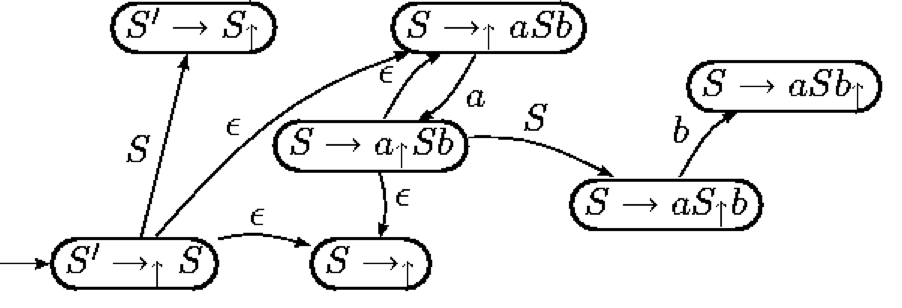
\epsfig{file=chapter_bottomup/nfa.eps, width=12cm}}

\end{figure}%
\lthtmlfigureZ
\lthtmlcheckvsize\clearpage}

{\newpage\clearpage
\lthtmlinlinemathA{tex2html_wrap_inline38881}%
$ aabb$%
\lthtmlinlinemathZ
\lthtmlcheckvsize\clearpage}

{\newpage\clearpage
\lthtmlinlinemathA{tex2html_wrap_inline38883}%
$ aaSbb$%
\lthtmlinlinemathZ
\lthtmlcheckvsize\clearpage}

{\newpage\clearpage
\lthtmlinlinemathA{tex2html_wrap_inline38885}%
$ aSb$%
\lthtmlinlinemathZ
\lthtmlcheckvsize\clearpage}

\stepcounter{section}
\stepcounter{subsection}
{\newpage\clearpage
\lthtmlinlinemathA{tex2html_wrap_indisplay38935}%
$\displaystyle do$%
\lthtmlindisplaymathZ
\lthtmlcheckvsize\clearpage}

{\newpage\clearpage
\lthtmlinlinemathA{tex2html_wrap_indisplay38937}%
$\displaystyle \  \ FIRST(X) = FIRST(X) \cup FIRST(Y_i) - \{ \epsilon \};$%
\lthtmlindisplaymathZ
\lthtmlcheckvsize\clearpage}

{\newpage\clearpage
\lthtmlinlinemathA{tex2html_wrap_indisplay38941}%
$\displaystyle mientras\  (\epsilon \in FIRST(Y_i)\  and\  (i \leq k))$%
\lthtmlindisplaymathZ
\lthtmlcheckvsize\clearpage}

{\newpage\clearpage
\lthtmlinlinemathA{tex2html_wrap_indisplay38943}%
$\displaystyle si\  (\epsilon \in FIRST(Y_k)\  and\  i > k)\  FIRST(X) = FIRST(X) \cup \{ \epsilon \}$%
\lthtmlindisplaymathZ
\lthtmlcheckvsize\clearpage}

{\newpage\clearpage
\lthtmlinlinemathA{tex2html_wrap_indisplay38963}%
$\displaystyle \  \ FIRST(\alpha) = FIRST(\alpha) \cup FIRST(X_i) - \{ \epsilon \};$%
\lthtmlindisplaymathZ
\lthtmlcheckvsize\clearpage}

{\newpage\clearpage
\lthtmlinlinemathA{tex2html_wrap_indisplay38967}%
$\displaystyle mientras\  (\epsilon \in FIRST(X_i)\  and\  (i \leq n))$%
\lthtmlindisplaymathZ
\lthtmlcheckvsize\clearpage}

{\newpage\clearpage
\lthtmlinlinemathA{tex2html_wrap_indisplay38969}%
$\displaystyle si\  (\epsilon \in FIRST(X_n)\  and\  i > n)\  FIRST(\alpha) = FIRST(X) \cup \{ \epsilon \}$%
\lthtmlindisplaymathZ
\lthtmlcheckvsize\clearpage}

{\newpage\clearpage
\lthtmlinlinemathA{tex2html_wrap_inline38990}%
$ Si\  A \rightarrow \alpha B$%
\lthtmlinlinemathZ
\lthtmlcheckvsize\clearpage}

{\newpage\clearpage
\lthtmlinlinemathA{tex2html_wrap_inline38992}%
$ A \rightarrow \alpha B \beta$%
\lthtmlinlinemathZ
\lthtmlcheckvsize\clearpage}

{\newpage\clearpage
\lthtmlinlinemathA{tex2html_wrap_inline38994}%
$ \epsilon \in FIRST(\beta)$%
\lthtmlinlinemathZ
\lthtmlcheckvsize\clearpage}

\stepcounter{subsection}
{\newpage\clearpage
\lthtmlinlinemathA{tex2html_wrap_inline38999}%
$ (Q, \Sigma, \delta, q_0)$%
\lthtmlinlinemathZ
\lthtmlcheckvsize\clearpage}

{\newpage\clearpage
\lthtmlinlinemathA{tex2html_wrap_inline39001}%
$ q_0$%
\lthtmlinlinemathZ
\lthtmlcheckvsize\clearpage}

{\newpage\clearpage
\lthtmlinlinemathA{tex2html_wrap_inline39005}%
$ \overline{\{q_0\}}$%
\lthtmlinlinemathZ
\lthtmlcheckvsize\clearpage}

{\newpage\clearpage
\lthtmlinlinemathA{tex2html_wrap_inline39007}%
$ \overline{\delta(\overline{\{q_0\}},a)}$%
\lthtmlinlinemathZ
\lthtmlcheckvsize\clearpage}

{\newpage\clearpage
\lthtmlinlinemathA{tex2html_wrap_inline39009}%
$ \overline{A}$%
\lthtmlinlinemathZ
\lthtmlcheckvsize\clearpage}

{\newpage\clearpage
\lthtmlinlinemathA{tex2html_wrap_inline39021}%
$ \overline{A} = \{ q \in Q\  /\   \exists q' \in Q\  :\  \hat{\delta}(q', \epsilon) = q \}$%
\lthtmlinlinemathZ
\lthtmlcheckvsize\clearpage}

{\newpage\clearpage
\lthtmlinlinemathA{tex2html_wrap_inline39023}%
$ \hat{\delta}$%
\lthtmlinlinemathZ
\lthtmlcheckvsize\clearpage}

{\newpage\clearpage
\lthtmlinlinemathA{tex2html_wrap_inline39025}%
$ \Sigma^*$%
\lthtmlinlinemathZ
\lthtmlcheckvsize\clearpage}

{\newpage\clearpage
\lthtmlinlinemathA{tex2html_wrap_indisplay39027}%
$\displaystyle \hat{\delta}(q, x) = \left \{ \begin{array}{ll}                          \delta(\hat{\delta}(q,y),a) & \mbox{si $x = ya$} \\q & \mbox{si $x = \epsilon$}                        \end{array}              \right.$%
\lthtmlindisplaymathZ
\lthtmlcheckvsize\clearpage}

{\newpage\clearpage
\lthtmlfigureA{figure15582}%
\begin{figure}\centerline{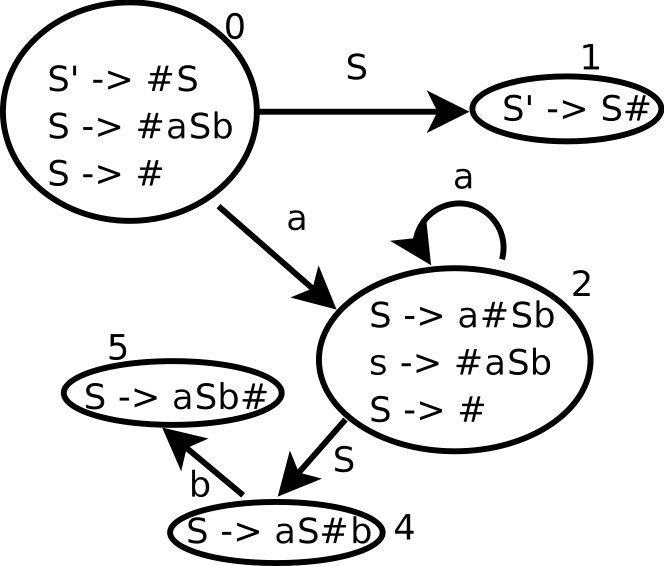
\epsfig{file=chapter_bottomup/dfa.eps, width=12cm}}

\end{figure}%
\lthtmlfigureZ
\lthtmlcheckvsize\clearpage}

{\newpage\clearpage
\lthtmlinlinemathA{tex2html_wrap_inline39044}%
$ I_i$%
\lthtmlinlinemathZ
\lthtmlcheckvsize\clearpage}

{\newpage\clearpage
\lthtmlinlinemathA{tex2html_wrap_inline39046}%
$ \delta_{| V \times Q} :  V \times Q \rightarrow Q$%
\lthtmlinlinemathZ
\lthtmlcheckvsize\clearpage}

{\newpage\clearpage
\lthtmlinlinemathA{tex2html_wrap_inline39048}%
$ goto(i, A) = \delta(A,I_i)$%
\lthtmlinlinemathZ
\lthtmlcheckvsize\clearpage}

{\newpage\clearpage
\lthtmlinlinemathA{tex2html_wrap_inline39050}%
$ \delta_{| \Sigma \times Q} :  \Sigma \times Q \rightarrow Q$%
\lthtmlinlinemathZ
\lthtmlcheckvsize\clearpage}

{\newpage\clearpage
\lthtmlinlinemathA{tex2html_wrap_inline39056}%
$ action(i, a) = shift\  \delta(a,I_i)$%
\lthtmlinlinemathZ
\lthtmlcheckvsize\clearpage}

{\newpage\clearpage
\lthtmlinlinemathA{tex2html_wrap_inline39060}%
$ A \rightarrow \alpha_\uparrow$%
\lthtmlinlinemathZ
\lthtmlcheckvsize\clearpage}

{\newpage\clearpage
\lthtmlinlinemathA{tex2html_wrap_inline39066}%
$ (s,a)$%
\lthtmlinlinemathZ
\lthtmlcheckvsize\clearpage}

{\newpage\clearpage
\lthtmlinlinemathA{tex2html_wrap_inline39074}%
$ action(i, a) = reduce\  A \rightarrow \alpha$%
\lthtmlinlinemathZ
\lthtmlcheckvsize\clearpage}

{\newpage\clearpage
\lthtmlinlinemathA{tex2html_wrap_inline39084}%
$ \exists S \begin{array}{c} *\\\Longrightarrow \\{\scriptstyle RM} \end{array} \beta A b x \begin{array}{c} *\\\Longrightarrow \\{\scriptstyle RM} \end{array}  
\beta \alpha b x = \gamma$%
\lthtmlinlinemathZ
\lthtmlcheckvsize\clearpage}

{\newpage\clearpage
\lthtmlinlinemathA{tex2html_wrap_inline39090}%
$ b \in FOLLOW(A)$%
\lthtmlinlinemathZ
\lthtmlcheckvsize\clearpage}

{\newpage\clearpage
\lthtmlinlinemathA{tex2html_wrap_inline39092}%
$ action(i, b) = reduce\  A \rightarrow \alpha$%
\lthtmlinlinemathZ
\lthtmlcheckvsize\clearpage}

{\newpage\clearpage
\lthtmlinlinemathA{tex2html_wrap_inline39103}%
$ (Q, V \cup \Sigma, \delta, I_0, F)$%
\lthtmlinlinemathZ
\lthtmlcheckvsize\clearpage}

{\newpage\clearpage
\lthtmlinlinemathA{tex2html_wrap_inline39105}%
$ C = \left \{ I_1, I_2, \cdots I_n \right \}$%
\lthtmlinlinemathZ
\lthtmlcheckvsize\clearpage}

{\newpage\clearpage
\lthtmlinlinemathA{tex2html_wrap_inline39113}%
$ goto(i,A) = \delta(I_i, A)$%
\lthtmlinlinemathZ
\lthtmlcheckvsize\clearpage}

{\newpage\clearpage
\lthtmlinlinemathA{tex2html_wrap_inline39119}%
$ A \rightarrow \alpha _\uparrow a \beta \in I_i$%
\lthtmlinlinemathZ
\lthtmlcheckvsize\clearpage}

{\newpage\clearpage
\lthtmlinlinemathA{tex2html_wrap_inline39121}%
$ \delta(I_i,a) = I_j$%
\lthtmlinlinemathZ
\lthtmlcheckvsize\clearpage}

{\newpage\clearpage
\lthtmlinlinemathA{tex2html_wrap_inline39125}%
$ action[i][a] = shift\  j$%
\lthtmlinlinemathZ
\lthtmlcheckvsize\clearpage}

{\newpage\clearpage
\lthtmlinlinemathA{tex2html_wrap_inline39127}%
$ S' \rightarrow S_\uparrow \in I_i$%
\lthtmlinlinemathZ
\lthtmlcheckvsize\clearpage}

{\newpage\clearpage
\lthtmlinlinemathA{tex2html_wrap_inline39129}%
$ action[i][\$] = accept$%
\lthtmlinlinemathZ
\lthtmlcheckvsize\clearpage}

{\newpage\clearpage
\lthtmlinlinemathA{tex2html_wrap_inline39131}%
$ A \rightarrow \alpha _\uparrow \in I_i$%
\lthtmlinlinemathZ
\lthtmlcheckvsize\clearpage}

{\newpage\clearpage
\lthtmlinlinemathA{tex2html_wrap_inline39133}%
$ \forall a \in\  FOLLOW(A):\  action[i][a] = reduce\  A \rightarrow \alpha$%
\lthtmlinlinemathZ
\lthtmlcheckvsize\clearpage}

{\newpage\clearpage
\lthtmlinlinemathA{tex2html_wrap_inline39135}%
$ error$%
\lthtmlinlinemathZ
\lthtmlcheckvsize\clearpage}

\stepcounter{section}
\stepcounter{section}
{\newpage\clearpage
\lthtmlinlinemathA{tex2html_wrap_inline39234}%
$ |x|$%
\lthtmlinlinemathZ
\lthtmlcheckvsize\clearpage}

\stepcounter{section}
\stepcounter{section}
\stepcounter{subsection}
\stepcounter{subsection}
\stepcounter{subsection}
\stepcounter{subsection}
\stepcounter{subsection}
\stepcounter{subsection}
\stepcounter{subsection}
\stepcounter{subsection}
\stepcounter{subsection}
\stepcounter{subsection}
\stepcounter{subsection}
\stepcounter{section}
\stepcounter{section}
\stepcounter{section}
\stepcounter{section}
\stepcounter{section}
{\newpage\clearpage
\lthtmlinlinemathA{tex2html_wrap_inline39277}%
$ G = (V, \Sigma, P, S)$%
\lthtmlinlinemathZ
\lthtmlcheckvsize\clearpage}

{\newpage\clearpage
\lthtmlinlinemathA{tex2html_wrap_inline39279}%
$ S \in V \cup \Sigma$%
\lthtmlinlinemathZ
\lthtmlcheckvsize\clearpage}

{\newpage\clearpage
\lthtmlinlinemathA{tex2html_wrap_inline39281}%
$ A \rightarrow X_1 X_2 \ldots X_n \in P$%
\lthtmlinlinemathZ
\lthtmlcheckvsize\clearpage}

{\newpage\clearpage
\lthtmlinlinemathA{tex2html_wrap_inline39283}%
$ X \in V \cup \Sigma$%
\lthtmlinlinemathZ
\lthtmlcheckvsize\clearpage}

{\newpage\clearpage
\lthtmlinlinemathA{tex2html_wrap_inline39285}%
$ X$%
\lthtmlinlinemathZ
\lthtmlcheckvsize\clearpage}

{\newpage\clearpage
\lthtmlinlinemathA{tex2html_wrap_inline39289}%
$ A \rightarrow X_1 \ldots X_n$%
\lthtmlinlinemathZ
\lthtmlcheckvsize\clearpage}

{\newpage\clearpage
\lthtmlinlinemathA{tex2html_wrap_inline39291}%
$ X_j$%
\lthtmlinlinemathZ
\lthtmlcheckvsize\clearpage}

\stepcounter{section}
\stepcounter{section}
\stepcounter{section}
\stepcounter{section}
{\newpage\clearpage
\lthtmlinlinemathA{tex2html_wrap_inline39303}%
$ B \rightarrow \beta_\uparrow \gamma$%
\lthtmlinlinemathZ
\lthtmlcheckvsize\clearpage}

{\newpage\clearpage
\lthtmlinlinemathA{tex2html_wrap_inline39307}%
$ a \in FOLLOW(A)$%
\lthtmlinlinemathZ
\lthtmlcheckvsize\clearpage}

{\newpage\clearpage
\lthtmlinlinemathA{tex2html_wrap_inline39309}%
$ a \in FIRST(\gamma)$%
\lthtmlinlinemathZ
\lthtmlcheckvsize\clearpage}

{\newpage\clearpage
\lthtmlinlinemathA{tex2html_wrap_inline39317}%
$ a \in FOLLOW(A) \cap FIRST(\gamma)$%
\lthtmlinlinemathZ
\lthtmlcheckvsize\clearpage}

{\newpage\clearpage
\lthtmlinlinemathA{tex2html_wrap_inline39319}%
$ FOLLOW(A) \cap FIRST(\gamma)$%
\lthtmlinlinemathZ
\lthtmlcheckvsize\clearpage}

\stepcounter{chapter}
\stepcounter{section}
{\newpage\clearpage
\lthtmlinlinemathA{tex2html_wrap_inline39323}%
$ -(-(4,5),2)$%
\lthtmlinlinemathZ
\lthtmlcheckvsize\clearpage}

{\newpage\clearpage
\lthtmlinlinemathA{tex2html_wrap_inline39325}%
$ -(4, -(5,2))$%
\lthtmlinlinemathZ
\lthtmlcheckvsize\clearpage}

{\newpage\clearpage
\lthtmlinlinemathA{tex2html_wrap_inline39327}%
$ E \rightarrow - E$%
\lthtmlinlinemathZ
\lthtmlcheckvsize\clearpage}

{\newpage\clearpage
\lthtmlinlinemathA{tex2html_wrap_inline39329}%
$ E \rightarrow E - E$%
\lthtmlinlinemathZ
\lthtmlcheckvsize\clearpage}

{\newpage\clearpage
\lthtmlinlinemathA{tex2html_wrap_inline39336}%
$ NUM + NUM \stackrel{NUM \leftarrow E}{\Longleftarrow} E + NUM \stackrel{NUM \leftarrow E}{\Longleftarrow} E + E \stackrel{E +E \leftarrow E}{\Longleftarrow} E
$%
\lthtmlinlinemathZ
\lthtmlcheckvsize\clearpage}

{\newpage\clearpage
\lthtmlinlinemathA{tex2html_wrap_inline39338}%
$ E \rightarrow E + E$%
\lthtmlinlinemathZ
\lthtmlcheckvsize\clearpage}

\stepcounter{section}
{\newpage\clearpage
\lthtmlinlinemathA{tex2html_wrap_inline39410}%
$ PV = \left \{ \delta \in (\Sigma \cup V)* :  \exists S \begin{array}{c} *\\\Longrightarrow \\{\scriptstyle RM} \end{array} \alpha\   y\  \delta\  es\  un\  prefijo\  de\   handle_2(\alpha) \right \}$%
\lthtmlinlinemathZ
\lthtmlcheckvsize\clearpage}

{\newpage\clearpage
\lthtmlinlinemathA{tex2html_wrap_inline39435}%
$ Alfabeto = V \cup \Sigma$%
\lthtmlinlinemathZ
\lthtmlcheckvsize\clearpage}

{\newpage\clearpage
\lthtmlinlinemathA{tex2html_wrap_inline39455}%
$ \delta(A \rightarrow \alpha _\uparrow B \beta, \epsilon) = B \rightarrow \gamma  \forall B \in  V$%
\lthtmlinlinemathZ
\lthtmlcheckvsize\clearpage}

{\newpage\clearpage
\lthtmlfigureA{figure17454}%
\begin{figure}
\end{figure}%
\lthtmlfigureZ
\lthtmlcheckvsize\clearpage}

\stepcounter{section}
\stepcounter{subsection}
\stepcounter{subsection}
{\newpage\clearpage
\lthtmlinlinemathA{tex2html_wrap_inline39638}%
$ \overline{A} = \{ q \in Q\  /\   \exists q' \in Q\  :\  \hat{\delta}(q, \epsilon) = q \}$%
\lthtmlinlinemathZ
\lthtmlcheckvsize\clearpage}

{\newpage\clearpage
\lthtmlinlinemathA{tex2html_wrap_inline39669}%
$ action(i, a) = \delta(a,I_i)$%
\lthtmlinlinemathZ
\lthtmlcheckvsize\clearpage}

\stepcounter{section}
\stepcounter{section}
\stepcounter{section}
\stepcounter{section}
\stepcounter{section}
\stepcounter{section}
\stepcounter{section}
{\newpage\clearpage
\lthtmlinlinemathA{tex2html_wrap_inline39869}%
$ \left \{ action_1\right \}$%
\lthtmlinlinemathZ
\lthtmlcheckvsize\clearpage}

{\newpage\clearpage
\lthtmlinlinemathA{tex2html_wrap_inline39873}%
$ A \rightarrow \alpha \left \{ action_1 \right \} \beta \left \{ action_2\right \}$%
\lthtmlinlinemathZ
\lthtmlcheckvsize\clearpage}

{\newpage\clearpage
\lthtmlinlinemathA{tex2html_wrap_inline39875}%
$ T$%
\lthtmlinlinemathZ
\lthtmlcheckvsize\clearpage}

{\newpage\clearpage
\lthtmlinlinemathA{tex2html_wrap_inline39877}%
$ A \rightarrow \alpha T \beta \left \{ action_2\right \}$%
\lthtmlinlinemathZ
\lthtmlcheckvsize\clearpage}

{\newpage\clearpage
\lthtmlinlinemathA{tex2html_wrap_inline39879}%
$ T \rightarrow \epsilon \left \{ action_1 \right \}$%
\lthtmlinlinemathZ
\lthtmlcheckvsize\clearpage}

\stepcounter{section}
{\newpage\clearpage
\lthtmlinlinemathA{tex2html_wrap_inline39882}%
$ A \rightarrow X_1 \ldots X_j$%
\lthtmlinlinemathZ
\lthtmlcheckvsize\clearpage}

{\newpage\clearpage
\lthtmlinlinemathA{tex2html_wrap_inline39884}%
$ _1$%
\lthtmlinlinemathZ
\lthtmlcheckvsize\clearpage}

{\newpage\clearpage
\lthtmlinlinemathA{tex2html_wrap_inline39886}%
$ \ldots$%
\lthtmlinlinemathZ
\lthtmlcheckvsize\clearpage}

{\newpage\clearpage
\lthtmlinlinemathA{tex2html_wrap_inline39888}%
$ _n$%
\lthtmlinlinemathZ
\lthtmlcheckvsize\clearpage}

{\newpage\clearpage
\lthtmlinlinemathA{tex2html_wrap_inline39890}%
$ X_{j+1} \ldots X_n$%
\lthtmlinlinemathZ
\lthtmlcheckvsize\clearpage}

\stepcounter{section}
\stepcounter{section}
{\newpage\clearpage
\lthtmlinlinemathA{tex2html_wrap_inline39920}%
$ X_m \ldots X_1 X_0 Y_1 \ldots  Y_n a_1 \ldots a_0$%
\lthtmlinlinemathZ
\lthtmlcheckvsize\clearpage}

{\newpage\clearpage
\lthtmlinlinemathA{tex2html_wrap_inline39922}%
$ B \rightarrow Y_1 \ldots  Y_n$%
\lthtmlinlinemathZ
\lthtmlcheckvsize\clearpage}

{\newpage\clearpage
\lthtmlinlinemathA{tex2html_wrap_inline39924}%
$ a_1 \ldots a_0$%
\lthtmlinlinemathZ
\lthtmlcheckvsize\clearpage}

{\newpage\clearpage
\lthtmlinlinemathA{tex2html_wrap_inline39926}%
$ Y_1$%
\lthtmlinlinemathZ
\lthtmlcheckvsize\clearpage}

{\newpage\clearpage
\lthtmlinlinemathA{tex2html_wrap_inline39928}%
$ Y_n$%
\lthtmlinlinemathZ
\lthtmlcheckvsize\clearpage}

{\newpage\clearpage
\lthtmlinlinemathA{tex2html_wrap_inline39930}%
$ X_0$%
\lthtmlinlinemathZ
\lthtmlcheckvsize\clearpage}

{\newpage\clearpage
\lthtmlinlinemathA{tex2html_wrap_inline39932}%
$ X_1$%
\lthtmlinlinemathZ
\lthtmlcheckvsize\clearpage}

{\newpage\clearpage
\lthtmlinlinemathA{tex2html_wrap_inline39934}%
$ X_m$%
\lthtmlinlinemathZ
\lthtmlcheckvsize\clearpage}

{\newpage\clearpage
\lthtmlinlinemathA{tex2html_wrap_inline39983}%
$ \Longrightarrow$%
\lthtmlinlinemathZ
\lthtmlcheckvsize\clearpage}

{\newpage\clearpage
\lthtmlinlinemathA{tex2html_wrap_inline39997}%
$ \Longleftarrow$%
\lthtmlinlinemathZ
\lthtmlcheckvsize\clearpage}

\stepcounter{section}
\stepcounter{section}
\stepcounter{section}
\stepcounter{section}
\stepcounter{section}
{\newpage\clearpage
\lthtmlinlinemathA{tex2html_wrap_inline40180}%
$ [$%
\lthtmlinlinemathZ
\lthtmlcheckvsize\clearpage}

{\newpage\clearpage
\lthtmlinlinemathA{tex2html_wrap_inline40182}%
$ ]$%
\lthtmlinlinemathZ
\lthtmlcheckvsize\clearpage}

{\newpage\clearpage
\lthtmlinlinemathA{tex2html_wrap_inline40236}%
$ ||$%
\lthtmlinlinemathZ
\lthtmlcheckvsize\clearpage}

{\newpage\clearpage
\lthtmlinlinemathA{tex2html_wrap_inline40248}%
$ <$%
\lthtmlinlinemathZ
\lthtmlcheckvsize\clearpage}

{\newpage\clearpage
\lthtmlinlinemathA{tex2html_wrap_inline40252}%
$ >$%
\lthtmlinlinemathZ
\lthtmlcheckvsize\clearpage}

{\newpage\clearpage
\lthtmlinlinemathA{tex2html_wrap_inline40256}%
$ <=$%
\lthtmlinlinemathZ
\lthtmlcheckvsize\clearpage}

{\newpage\clearpage
\lthtmlinlinemathA{tex2html_wrap_inline40260}%
$ >=$%
\lthtmlinlinemathZ
\lthtmlcheckvsize\clearpage}

{\newpage\clearpage
\lthtmlinlinemathA{tex2html_wrap_inline40280}%
$ ++$%
\lthtmlinlinemathZ
\lthtmlcheckvsize\clearpage}

{\newpage\clearpage
\lthtmlinlinemathA{tex2html_wrap_inline40284}%
$ --$%
\lthtmlinlinemathZ
\lthtmlcheckvsize\clearpage}

{\newpage\clearpage
\lthtmlinlinemathA{tex2html_wrap_inline40395}%
$ E_1$%
\lthtmlinlinemathZ
\lthtmlcheckvsize\clearpage}

{\newpage\clearpage
\lthtmlinlinemathA{tex2html_wrap_inline40397}%
$ E_2$%
\lthtmlinlinemathZ
\lthtmlcheckvsize\clearpage}

\stepcounter{section}
\stepcounter{subsection}
\stepcounter{subsection}
\stepcounter{subsection}
\stepcounter{subsection}
\stepcounter{subsection}
\stepcounter{subsection}
\stepcounter{section}
\stepcounter{section}
\stepcounter{section}
\stepcounter{section}
\stepcounter{section}
\stepcounter{section}
\stepcounter{section}
\stepcounter{section}
\stepcounter{section}
\stepcounter{section}
\stepcounter{paragraph}
\stepcounter{section}
\stepcounter{chapter}
\stepcounter{section}
\stepcounter{paragraph}
\stepcounter{paragraph}
\stepcounter{paragraph}
\stepcounter{paragraph}
\stepcounter{paragraph}
{\newpage\clearpage
\lthtmlinlinemathA{tex2html_wrap_inline40511}%
$ List \rightarrow \epsilon$%
\lthtmlinlinemathZ
\lthtmlcheckvsize\clearpage}

{\newpage\clearpage
\lthtmlinlinemathA{tex2html_wrap_inline40513}%
$ list \rightarrow list\  expr$%
\lthtmlinlinemathZ
\lthtmlcheckvsize\clearpage}

\stepcounter{section}
\stepcounter{section}
{\newpage\clearpage
\lthtmlinlinemathA{tex2html_wrap_inline40562}%
$ |\alpha|$%
\lthtmlinlinemathZ
\lthtmlcheckvsize\clearpage}

{\newpage\clearpage
\lthtmlinlinemathA{tex2html_wrap_inline40564}%
$ \rightarrow \alpha$%
\lthtmlinlinemathZ
\lthtmlcheckvsize\clearpage}

{\newpage\clearpage
\lthtmlinlinemathA{tex2html_wrap_inline40570}%
$ \cdots$%
\lthtmlinlinemathZ
\lthtmlcheckvsize\clearpage}

\stepcounter{section}
{\newpage\clearpage
\lthtmlinlinemathA{tex2html_wrap_inline40602}%
$ ABC$%
\lthtmlinlinemathZ
\lthtmlcheckvsize\clearpage}

{\newpage\clearpage
\lthtmlinlinemathA{tex2html_wrap_inline40604}%
$ t_1 \rightarrow \epsilon$%
\lthtmlinlinemathZ
\lthtmlcheckvsize\clearpage}

{\newpage\clearpage
\lthtmlinlinemathA{tex2html_wrap_inline40606}%
$ t_2 \rightarrow \epsilon$%
\lthtmlinlinemathZ
\lthtmlcheckvsize\clearpage}

{\newpage\clearpage
\lthtmlinlinemathA{tex2html_wrap_inline40608}%
$ s \rightarrow x t_1 s$%
\lthtmlinlinemathZ
\lthtmlcheckvsize\clearpage}

{\newpage\clearpage
\lthtmlinlinemathA{tex2html_wrap_inline40610}%
$ x \rightarrow A t_2 x$%
\lthtmlinlinemathZ
\lthtmlcheckvsize\clearpage}

{\newpage\clearpage
\lthtmlinlinemathA{tex2html_wrap_inline40642}%
$ FOLLOW(\verb|$$2|)$%
\lthtmlinlinemathZ
\lthtmlcheckvsize\clearpage}

\stepcounter{section}
{\newpage\clearpage
\lthtmlinlinemathA{tex2html_wrap_inline40684}%
$ \uparrow$%
\lthtmlinlinemathZ
\lthtmlcheckvsize\clearpage}

\stepcounter{section}
{\newpage\clearpage
\lthtmldisplayA{displaymath40692}%
\begin{displaymath}
\begin{array}{lll}
Construct         & EBNF & yacc\  input\\
\hline
optional\  sequence & x:\{y\}   & \verb|x : /* null */             |\\
                   &           & \verb|  | x y  { yyerrok; }      |\\
                   &           & \verb|  | x error                |\\
\hline
sequence          & x:y\{y\}  & \verb|x : y                      |\\
                  &           & \verb|  | xy   { yyerrok; }      |\\
                &           & \verb|  | error                  |\\
                &           & \verb|  | x error                |\\
\hline
list              & x:y\{Ty\} & \verb|x : y                       |\\
                  &           & \verb|  | x T y { yyerrok; }      |\\
                &           & \verb|  | error                   |\\
                &           & \verb|  | x error                 |\\
                &           & \verb|  | x error y { yyerrok; }  |\\
                &           & \verb|  | x  T error              |\\
\hline
\end{array}
\end{displaymath}%
\lthtmldisplayZ
\lthtmlcheckvsize\clearpage}

\stepcounter{chapter}
\stepcounter{chapter}
\stepcounter{section}
\stepcounter{chapter}
\stepcounter{chapter}
\stepcounter{chapter}
\stepcounter{chapter}
\stepcounter{part}
\stepcounter{chapter}
\stepcounter{section}
\stepcounter{subsection}
\stepcounter{section}
\stepcounter{subsection}

\end{document}
